\DocumentMetadata{%
 %  uncompress, %only for debugging!!
  pdfversion=2.0,
  testphase={phase-II, tabular, graphic}%
  % testphase={phase-II,math, tabular, graphic}% TOC Does not work
  % testphase={phase-III,math}% TOC works
}
\tagpdfsetup{activate, tabsorder=structure}
% Use the following to fix bug in November 2023 download of LaTeX
\ExplSyntaxOn
\cs_generate_variant:Nn\__tag_prop_gput:Nnn{cnx}
\ExplSyntaxOff
\documentclass[11pt,
  english,
  letterpaper,
]{article}
\usepackage{sa4ss}
\usepackage{amsmath,amssymb,array}
\usepackage{booktabs}

% From tagged-template.latex
\usepackage{lmodern}
\usepackage{ifxetex,ifluatex}
\ifnum 0\ifxetex 1\fi\ifluatex 1\fi=0 % if pdftex
  \usepackage[T1]{fontenc}
  \usepackage[utf8]{inputenc}
  \usepackage{textcomp} % provide euro and other symbols
\else % if luatex or xetex
  \usepackage{unicode-math}
  \defaultfontfeatures{Scale=MatchLowercase}
  \defaultfontfeatures[\rmfamily]{Ligatures=TeX,Scale=1}
\fi

% Use upquote if available, for straight quotes in verbatim environments
\IfFileExists{upquote.sty}{\usepackage{upquote}}{}
\IfFileExists{microtype.sty}{% use microtype if available
  \usepackage[]{microtype}
  \UseMicrotypeSet[protrusion]{basicmath} % disable protrusion for tt fonts
}{}
\makeatletter
\@ifundefined{KOMAClassName}{% if non-KOMA class
  \IfFileExists{parskip.sty}{%
    \usepackage{parskip}
  }{% else
    \setlength{\parindent}{0pt}
    \setlength{\parskip}{6pt plus 2pt minus 1pt}}
}{% if KOMA class
  \KOMAoptions{parskip=half}}
\makeatother
\usepackage{xcolor}
\IfFileExists{xurl.sty}{\usepackage{xurl}}{} % add URL line breaks if available
\hypersetup{
  pdftitle={Status of petrale sole (Eopsetta jordani) along the US West coast in 2023},
  pdflang={en},
  hidelinks,
  pdfcreator={LaTeX via pandoc}}
\urlstyle{same} % disable monospaced font for URLs
\usepackage{longtable}
% Correct order of tables after \paragraph or \subparagraph
\usepackage{etoolbox}
\makeatletter
\patchcmd\longtable{\par}{\if@noskipsec\mbox{}\fi\par}{}{}
\makeatother
% Allow footnotes in longtable head/foot
\IfFileExists{footnotehyper.sty}{\usepackage{footnotehyper}}{\usepackage{footnote}}
\makesavenoteenv{longtable}
\usepackage{graphicx}
\makeatletter
\def\maxwidth{\ifdim\Gin@nat@width>\linewidth\linewidth\else\Gin@nat@width\fi}
\def\maxheight{\ifdim\Gin@nat@height>\textheight\textheight\else\Gin@nat@height\fi}
\makeatother
% Scale images if necessary, so that they will not overflow the page
% margins by default, and it is still possible to overwrite the defaults
% using explicit options in \includegraphics[width, height, ...]{}
\setkeys{Gin}{width=\maxwidth,height=\maxheight,keepaspectratio}
% Set default figure placement to htbp
\makeatletter
\def\fps@figure{htbp}
\makeatother
\setlength{\emergencystretch}{3em} % prevent overfull lines
\providecommand{\tightlist}{%
  \setlength{\itemsep}{0pt}\setlength{\parskip}{0pt}}
\setcounter{secnumdepth}{5}
\ifxetex
  % Load polyglossia as late as possible: uses bidi with RTL langages (e.g. Hebrew, Arabic)
  \usepackage{polyglossia}
  \setmainlanguage[]{}
\else
  \usepackage[shorthands=off,main=english]{babel}
\fi

%Define cslreferences environment, required by pandoc 2.8
%https://github.com/rstudio/rmarkdown/issues/1649
\newlength{\csllabelwidth}
\setlength{\csllabelwidth}{3em}
\newlength{\cslhangindent}
\setlength{\cslhangindent}{1.5em}
% for Pandoc 2.8 to 2.10.1
\newenvironment{cslreferences}%
  {}%
  {\par}
% For Pandoc 2.11+
\newenvironment{CSLReferences}[2] % #1 hanging-ident, #2 entry spacing
 {% don't indent paragraphs
  \setlength{\parindent}{0pt}
  % turn on hanging indent if param 1 is 1
  \ifodd #1 \everypar{\setlength{\hangindent}{\cslhangindent}}\ignorespaces\fi
  % set entry spacing
  \ifnum #2 > 0
  \setlength{\parskip}{#2\baselineskip}
  \fi
 }%
 {}
\usepackage{calc}  % for \widthof, \maxof in minipage
\newcommand{\CSLBlock}[1]{#1\hfill\break}
\newcommand{\CSLLeftMargin}[1]{\parbox[t]{\csllabelwidth}{#1}}
\newcommand{\CSLRightInline}[1]{\parbox[t]{\linewidth - \csllabelwidth}{#1}\break}
\newcommand{\CSLIndent}[1]{\hspace{\cslhangindent}#1}


\providecommand{\tightlist}{%
  \setlength{\itemsep}{0pt}\setlength{\parskip}{0pt}}


\date{}
\newcommand{\trTitle}{Status of petrale sole (\emph{Eopsetta jordani}) along the US West coast in 2023}
\newcommand{\trYear}{2022}
\newcommand{\trMonth}{December}
\newcommand{\trAuthsLong}{truetrue}
\newcommand{\trAuthsBack}{Taylor, I.G., V. Gertseva}
\newcommand{\trCitation}{
\begin{hangparas}{1em}{1}
\trAuthsBack{}. \trYear{}. \trTitle{}. \glsentrylong{pfmc}, Portland, Oregon. \pageref{LastPage}{}\,p.
\end{hangparas}}

\begin{document}

%%%%% Frontmatter %%%%%

% Footnote symbols in front matter
\renewcommand*{\thefootnote}{\fnsymbol{footnote}}

\small
\thispagestyle{empty}
\pagenumbering{roman}
\noindent
\begin{center}
\title{Status of petrale sole (\emph{Eopsetta jordani}) along the US West coast in 2023}
% \textnormal{\MakeTextUppercase{\trTitle{}}}
\vspace{1.5cm}
{\Large\textbf\newline{Status of petrale sole (\emph{Eopsetta jordani}) along the US West coast in 2023}}
\vfill
by\\
Ian G. Taylor\textsuperscript{1}\\
Vladlena Gertseva\textsuperscript{1}\vfill
\textsuperscript{1}Northwest Fisheries Science Center, U.S. Department of Commerce, National Oceanic and Atmospheric Administration, National Marine Fisheries Service, 2725 Montlake Boulevard East, Seattle, Washington 98112\vfill
\trMonth{} \trYear{}
\end{center}
\clearpage

% Fourth page: Colophon
\thispagestyle{empty}
\vspace*{\fill}
\begin{center}
\copyright{} \glsentrylong{pfmc}, \trYear{}\\
\end{center}
\par
\bigskip
\noindent
Correct citation for this publication:
\bigskip
\par
\trCitation{}
\clearpage

% Add TOC to pdf bookmarks (clickable pdf)
\pdfbookmark[1]{\contentsname}{toc}

% Table of contents page, lists of figures and tables
\tableofcontents\clearpage
\label{TRlastRoman}
\clearpage

% Table of contents
\newpage
\thispagestyle{empty} % to remove page number

% Settings for the main document
\pagenumbering{arabic}  % Regular page numbers
\pagestyle{plain}  % No page number on first page of main document, use 'empty'
\renewcommand*{\thefootnote}{\arabic{footnote}}  % Back to numeric footnotes
\setcounter{footnote}{0}  % And start at 1
\renewcommand{\headrulewidth}{0.5pt}
\renewcommand{\footrulewidth}{0.5pt}
%\pagestyle{fancy}\fancyhead[c]{Draft: Do not cite or circulate}

\newcommand{\lt}{\ensuremath <}
\newcommand{\gt}{\ensuremath >}

\pagebreak
\pagenumbering{roman}
\setcounter{page}{1}

\renewcommand{\thetable}{\roman{table}}
\renewcommand{\thefigure}{\roman{figure}}

\setlength\parskip{0.5em plus 0.1em minus 0.2em}

\hypertarget{executive-summary}{%
\section*{Executive summary}\label{executive-summary}}
\addcontentsline{toc}{section}{Executive summary}

\hypertarget{stock}{%
\subsection*{Stock}\label{stock}}
\addcontentsline{toc}{subsection}{Stock}

This assessment reports the status of petrale sole (\emph{Eopsetta jordani}) off the US West coast using data through 2022.

\hypertarget{catches}{%
\subsection*{Catches}\label{catches}}
\addcontentsline{toc}{subsection}{Catches}

Adding text here for example. trends and current levels. Include Table for last 10 years. Include Figure with long-term estimates.

\clearpage

\begingroup\fontsize{10}{12}\selectfont
\begingroup\fontsize{10}{12}\selectfont

\begin{longtable}[t]{r>{\centering\arraybackslash}p{1.57cm}>{\centering\arraybackslash}p{1.57cm}>{\centering\arraybackslash}p{1.57cm}>{\centering\arraybackslash}p{1.57cm}>{\centering\arraybackslash}p{1.57cm}>{\centering\arraybackslash}p{1.57cm}}
\caption{\label{tab:removalsES}Recent landings by fleet, total landings summed across fleets, and the total mortality including discards.}\\
\toprule
Year & WinterN & SummerN & WinterS & SummerS & Total Landings & Total Dead\\
\midrule
\endfirsthead
\caption[]{Recent landings by fleet, total landings summed across fleets, and the total mortality including discards. \textit{(continued)}}\\
\toprule
Year & WinterN & SummerN & WinterS & SummerS & Total Landings & Total Dead\\
\midrule
\endhead

\endfoot
\bottomrule
\endlastfoot
2013 & 512.96 & 1044.72 & 130.10 & 279.58 & 1967.36 & 1994.60\\
2014 & 852.91 & 860.57 & 273.39 & 386.05 & 2372.92 & 2391.25\\
2015 & 1039.95 & 1076.66 & 215.38 & 354.03 & 2686.02 & 2703.64\\
2016 & 864.54 & 1168.42 & 237.49 & 235.49 & 2505.94 & 2522.13\\
2017 & 1142.29 & 1270.92 & 201.09 & 393.38 & 3007.68 & 3025.18\\
2018 & 957.29 & 1262.43 & 218.04 & 402.22 & 2839.98 & 2856.18\\
2019 & 859.05 & 1207.49 & 94.86 & 442.10 & 2603.50 & 2670.71\\
2020 & 678.88 & 821.81 & 197.40 & 346.01 & 2044.10 & 2092.98\\
2021 & 858.05 & 1107.98 & 315.58 & 460.50 & 2742.11 & 2806.73\\
2022 & 611.13 & 1155.22 & 323.74 & 514.22 & 2604.32 & 2676.86\\*
\end{longtable}
\endgroup{}
\endgroup{}


\begin{figure}
\centering
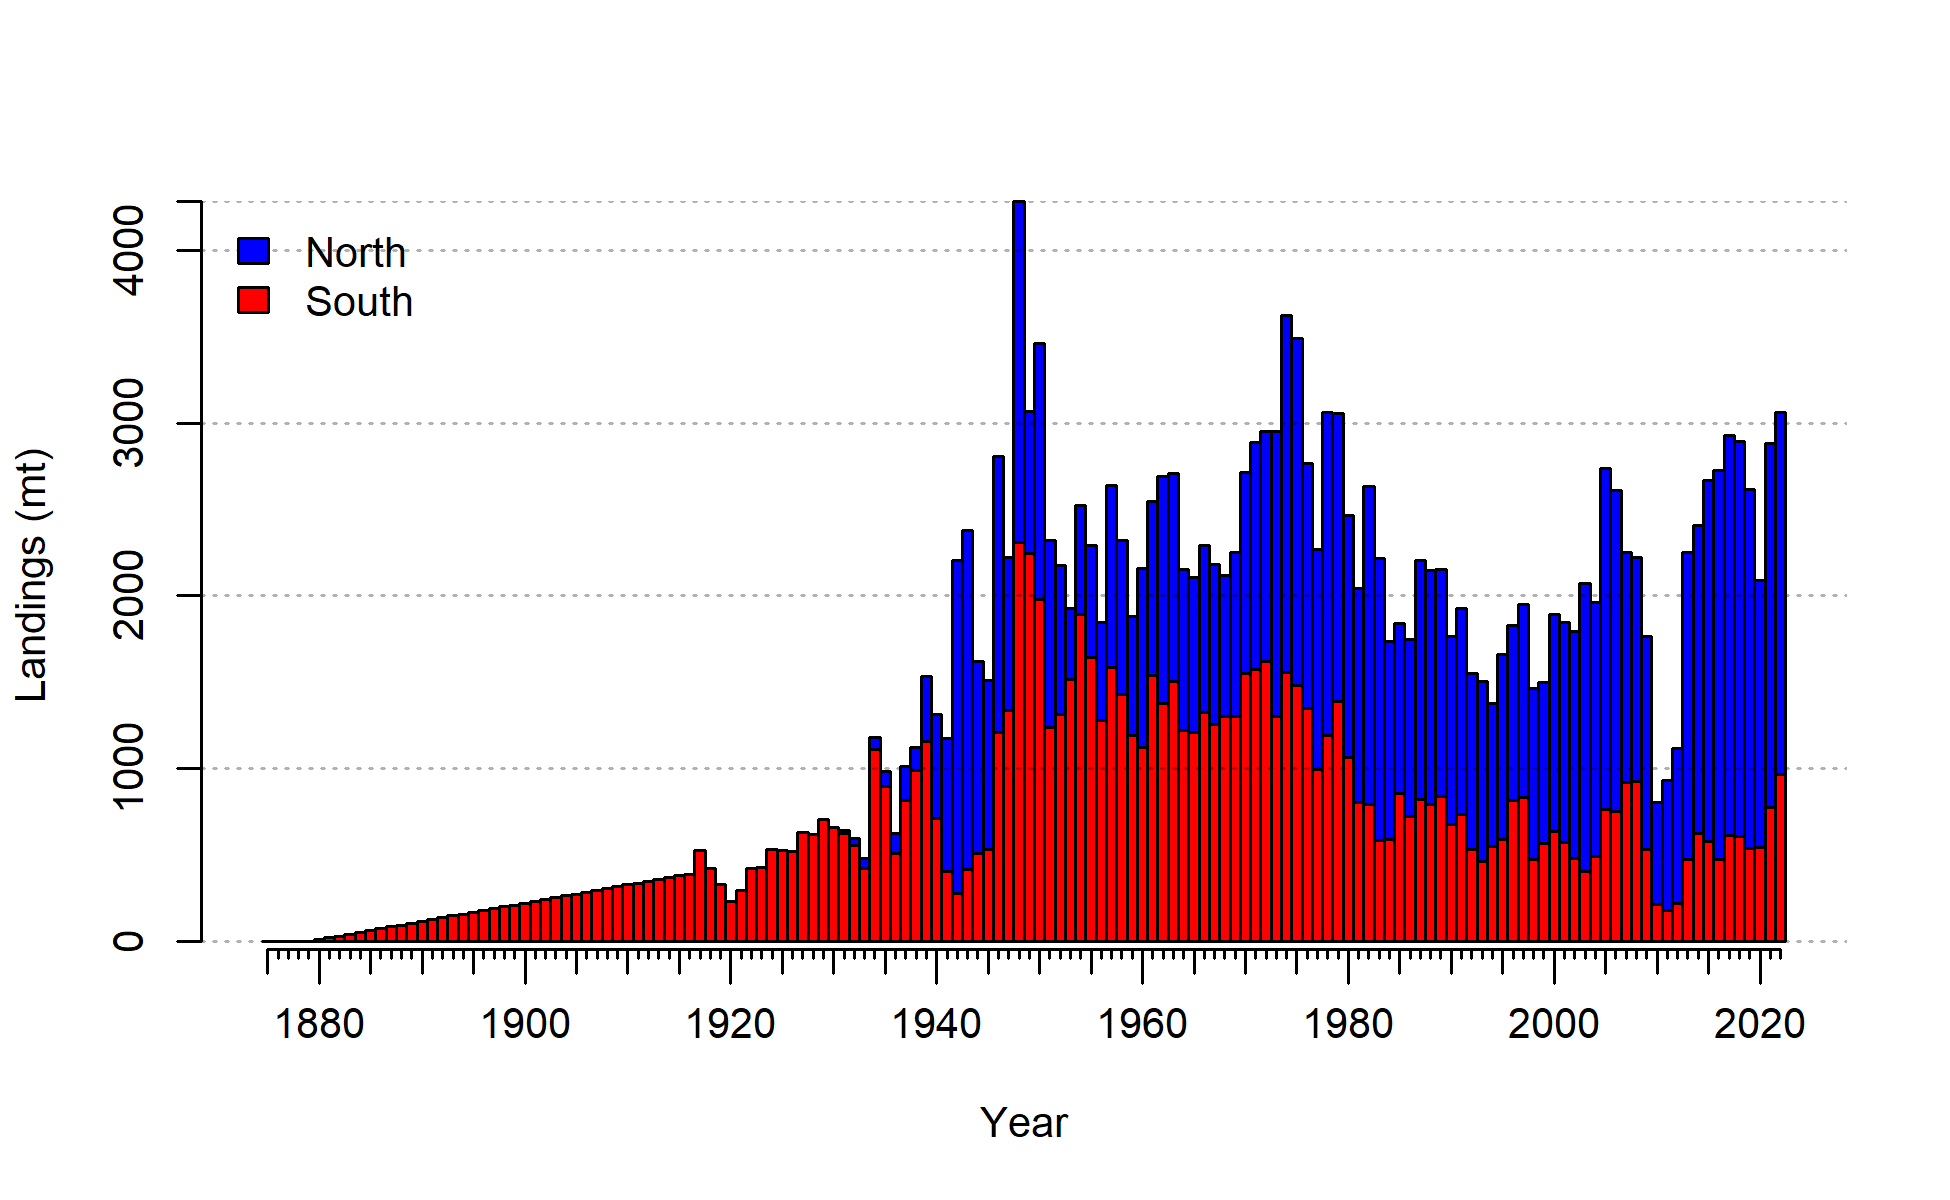
\includegraphics[width=1\textwidth,height=1\textheight]{../models/2023.005.001/plots/catch2 landings stacked.png}
\caption{Landings by fleet used in the base model where catches in metric tons by fleet are stacked.\label{fig:es-catch}}
\end{figure}

\clearpage

\hypertarget{data-and-assessment}{%
\subsection*{Data and assessment}\label{data-and-assessment}}
\addcontentsline{toc}{subsection}{Data and assessment}

This assessment uses the stock assessment framework Stock Synthesis

\begin{verbatim}
[1] "3.30.20.00"
\end{verbatim}

(SS3).

Replace text with date of last assessment, type of assessment model, data available, new information, and information lacking.

\hypertarget{stock-biomass-and-dynamics}{%
\subsection*{Stock biomass and dynamics}\label{stock-biomass-and-dynamics}}
\addcontentsline{toc}{subsection}{Stock biomass and dynamics}

Replace text with trends and current levels relative to virgin or historic levels and description of uncertainty. Include Table for last 10 years. Include Figure with long-term estimates.

\begingroup\fontsize{10}{12}\selectfont
\begingroup\fontsize{10}{12}\selectfont

\begin{longtable}[t]{r>{\centering\arraybackslash}p{1.57cm}>{\centering\arraybackslash}p{1.57cm}>{\centering\arraybackslash}p{1.57cm}>{\centering\arraybackslash}p{1.57cm}>{\centering\arraybackslash}p{1.57cm}>{\centering\arraybackslash}p{1.57cm}}
\caption{\label{tab:ssbES}Estimated recent trend in spawning biomass and the fraction unfished and the 95 percent intervals.}\\
\toprule
Year & Spawning Biomass (mt) & Lower Interval & Upper Interval & Fraction Unfished & Lower Interval & Upper Interval\\
\midrule
\endfirsthead
\caption[]{Estimated recent trend in spawning biomass and the fraction unfished and the 95 percent intervals. \textit{(continued)}}\\
\toprule
Year & Spawning Biomass (mt) & Lower Interval & Upper Interval & Fraction Unfished & Lower Interval & Upper Interval\\
\midrule
\endhead

\endfoot
\bottomrule
\endlastfoot
2013 & 9373.01 & 7761.70 & 10984.32 & 0.25 & 0.17 & 0.33\\
2014 & 11477.70 & 9515.93 & 13439.47 & 0.31 & 0.21 & 0.41\\
2015 & 12959.50 & 10769.79 & 15149.21 & 0.35 & 0.24 & 0.46\\
2016 & 13702.80 & 11393.77 & 16011.83 & 0.37 & 0.25 & 0.48\\
2017 & 14239.60 & 11846.93 & 16632.27 & 0.38 & 0.27 & 0.50\\
2018 & 14312.80 & 11840.48 & 16785.12 & 0.38 & 0.27 & 0.50\\
2019 & 14261.80 & 11715.59 & 16808.01 & 0.38 & 0.27 & 0.50\\
2020 & 14086.40 & 11469.83 & 16702.97 & 0.38 & 0.27 & 0.49\\
2021 & 13968.80 & 11287.84 & 16649.76 & 0.38 & 0.27 & 0.49\\
2022 & 13112.00 & 10371.64 & 15852.36 & 0.35 & 0.25 & 0.46\\
2023 & 12173.60 & 9363.27 & 14983.93 & 0.33 & 0.23 & 0.43\\*
\end{longtable}
\endgroup{}
\endgroup{}


\begin{figure}
\centering
\includegraphics[width=1\textwidth,height=1\textheight]{../models/2023.005.001/plots/ts7_Spawning_biomass_(mt)_with_95_asymptotic_intervals_intervals.png}
\caption{Estimated time series of spawning output (circles and line: median; light broken lines: 95 percent intervals) for the base model.\label{fig:es-ssb}}
\end{figure}

\begin{figure}
\centering
\includegraphics[width=1\textwidth,height=1\textheight]{../models/2023.005.001/plots/ts9_Relative_spawning_biomass_intervals.png}
\caption{Estimated time series of fraction of unfished spawning output (circles and line: median; light broken lines: 95 percent intervals) for the base model.\label{fig:es-depl}}
\end{figure}

\clearpage

\hypertarget{recruitment}{%
\subsection*{Recruitment}\label{recruitment}}
\addcontentsline{toc}{subsection}{Recruitment}

Replace text with trends and current levels relative to virgin or historic levels and description of uncertainty. Include Table for last 10 years. Include Figure with long-term estimates.

\begingroup\fontsize{10}{12}\selectfont
\begingroup\fontsize{10}{12}\selectfont

\begin{longtable}[t]{r>{\centering\arraybackslash}p{1.57cm}>{\centering\arraybackslash}p{1.57cm}>{\centering\arraybackslash}p{1.57cm}>{\centering\arraybackslash}p{1.57cm}>{\centering\arraybackslash}p{1.57cm}>{\centering\arraybackslash}p{1.57cm}}
\caption{\label{tab:recrES}Estimated recent trend in recruitment and recruitment deviations and the 95 percent intervals.}\\
\toprule
Year & Recruitment & Lower Interval & Upper Interval & Recruitment Deviations & Lower Interval & Upper Interval\\
\midrule
\endfirsthead
\caption[]{Estimated recent trend in recruitment and recruitment deviations and the 95 percent intervals. \textit{(continued)}}\\
\toprule
Year & Recruitment & Lower Interval & Upper Interval & Recruitment Deviations & Lower Interval & Upper Interval\\
\midrule
\endhead

\endfoot
\bottomrule
\endlastfoot
2013 & 13111.5 & 8088.64 & 21253.43 & -0.23 & -0.60 & 0.14\\
2014 & 13152.7 & 7955.88 & 21744.11 & -0.25 & -0.65 & 0.15\\
2015 & 12427.0 & 6974.63 & 22141.73 & -0.32 & -0.81 & 0.17\\
2016 & 15953.7 & 8289.89 & 30702.54 & -0.10 & -0.67 & 0.47\\
2017 & 15955.0 & 7320.70 & 34772.93 & -0.12 & -0.85 & 0.61\\
2018 & 18354.9 & 8071.63 & 41739.06 & 0.00 & -0.78 & 0.78\\
2019 & 18312.3 & 8058.62 & 41612.60 & 0.00 & -0.78 & 0.78\\
2020 & 18489.7 & 8129.94 & 42050.61 & 0.00 & -0.78 & 0.78\\
2021 & 18630.2 & 8185.88 & 42400.35 & 0.00 & -0.78 & 0.78\\
2022 & 18751.5 & 8233.21 & 42707.36 & 0.00 & -0.78 & 0.78\\
2023 & 18861.5 & 8275.15 & 42990.89 & 0.00 & -0.78 & 0.78\\*
\end{longtable}
\endgroup{}
\endgroup{}


\begin{figure}
\centering
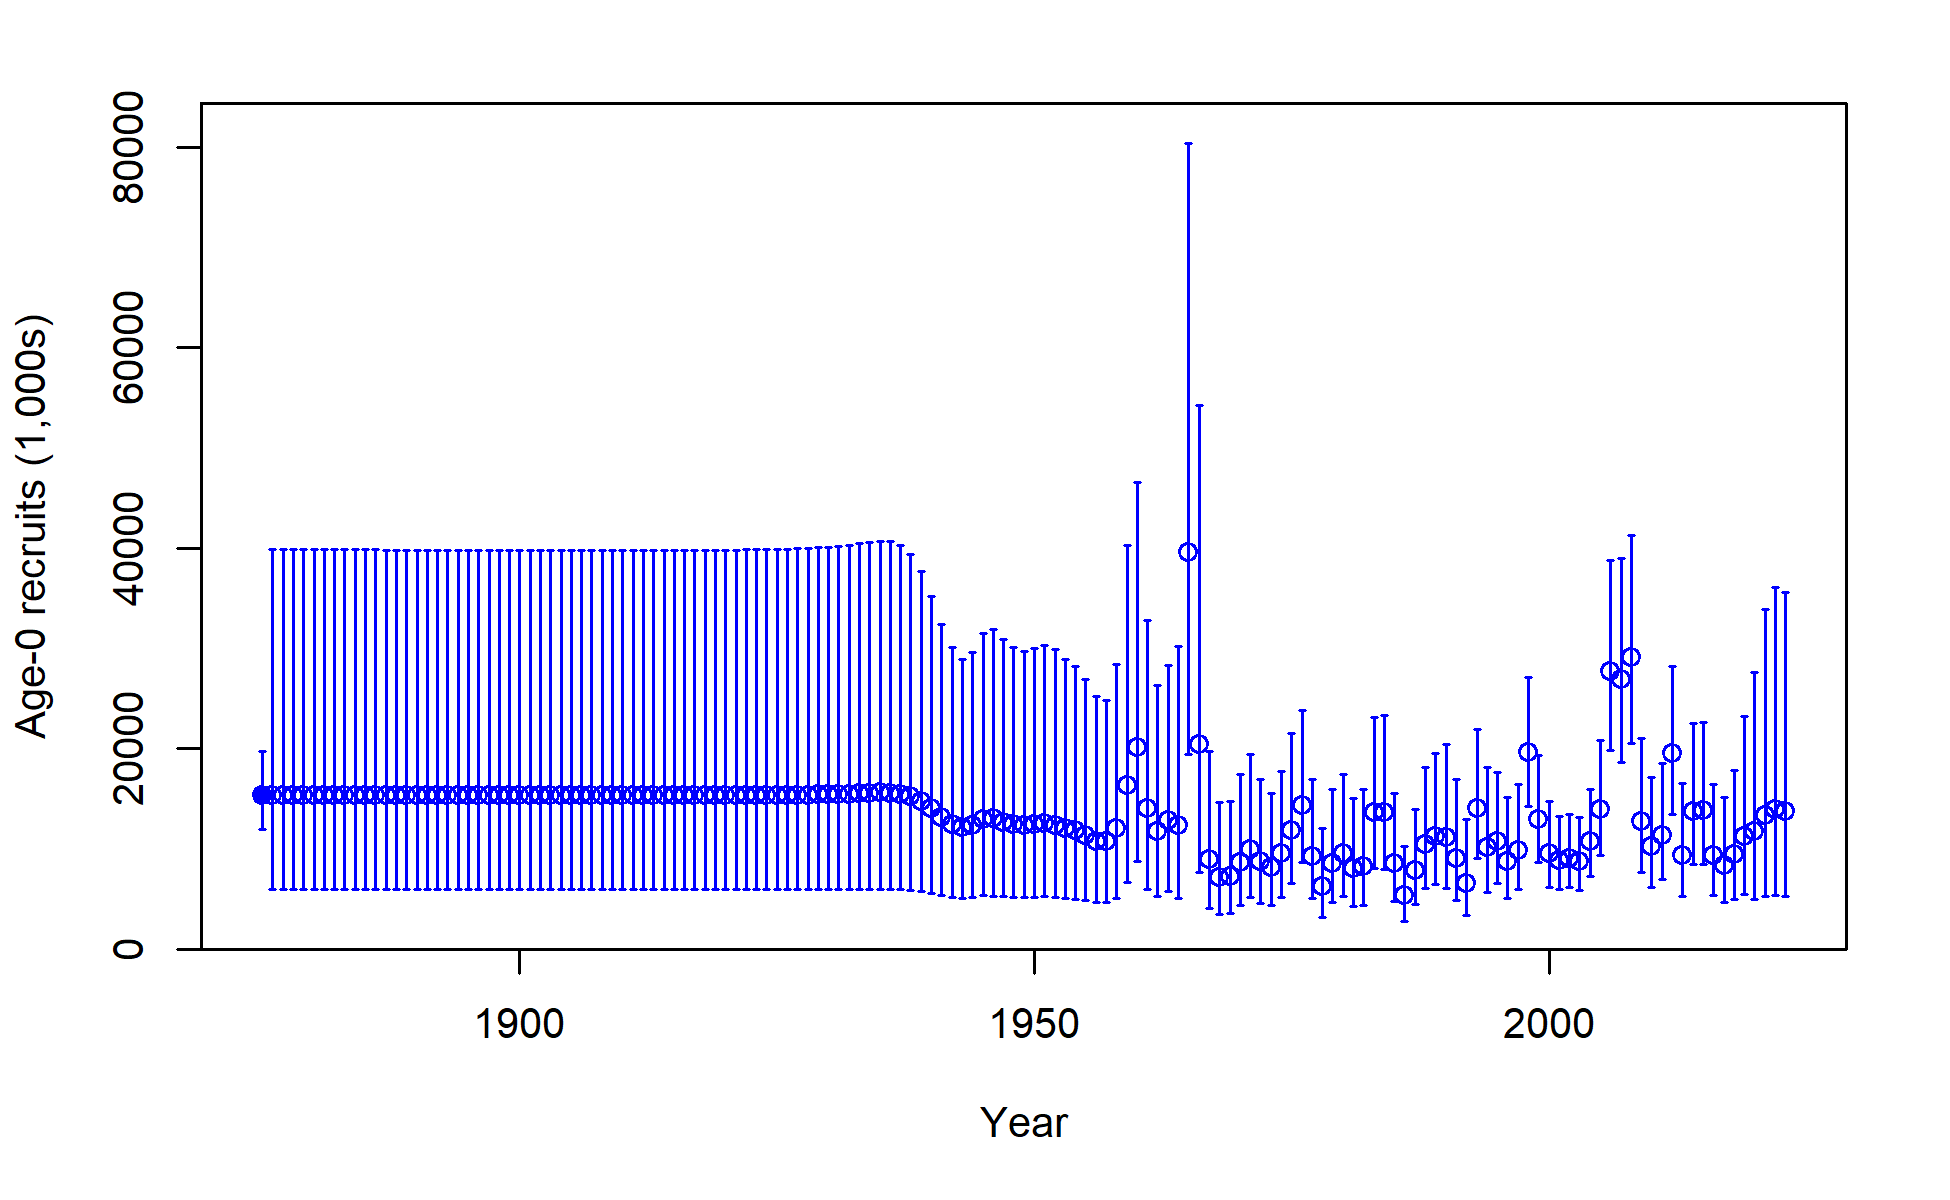
\includegraphics[width=1\textwidth,height=1\textheight]{../models/2023.005.001/plots/ts11_Age-0_recruits_(1000s)_with_95_asymptotic_intervals.png}
\caption{Estimated time series of age-0 recruits (1000s) for the base model with 95 percent intervals.\label{fig:es-recruits}}
\end{figure}

\begin{figure}
\centering
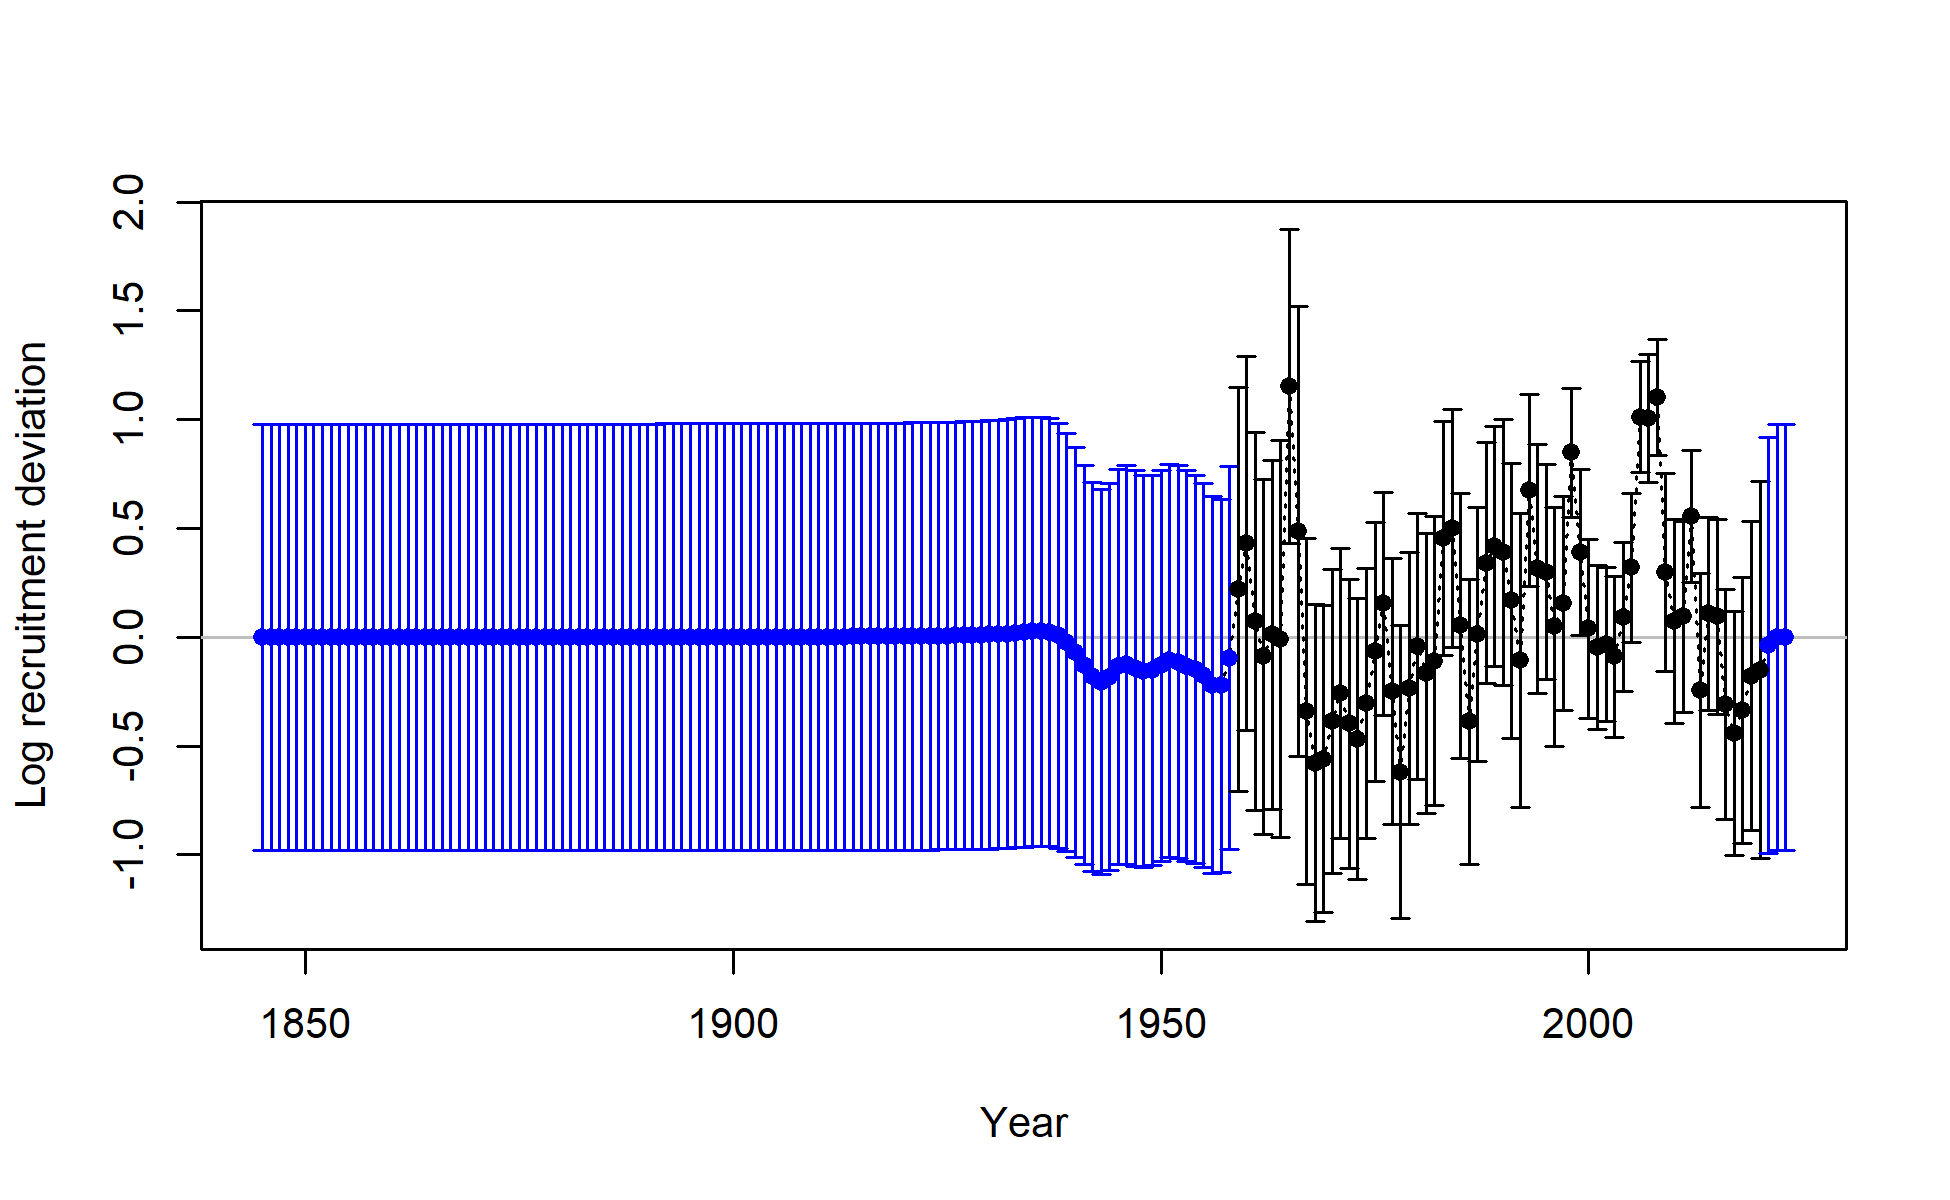
\includegraphics[width=1\textwidth,height=1\textheight]{../models/2023.005.001/plots/recdevs2_withbars.png}
\caption{Estimated time series of recruitment deviations.\label{fig:es-rec-devs}}
\end{figure}

\clearpage

\hypertarget{exploitation-status}{%
\subsection*{Exploitation status}\label{exploitation-status}}
\addcontentsline{toc}{subsection}{Exploitation status}

Replace text with total catch divided by exploitable biomass or SPR harvest rate. Include Table for last 10 years. Include Figure with trend in f relative to target vs.~trend in biomass relative to the target.

\begingroup\fontsize{10}{12}\selectfont
\begingroup\fontsize{10}{12}\selectfont

\begin{longtable}[t]{r>{\centering\arraybackslash}p{1.57cm}>{\centering\arraybackslash}p{1.57cm}>{\centering\arraybackslash}p{1.57cm}>{\centering\arraybackslash}p{1.57cm}>{\centering\arraybackslash}p{1.57cm}>{\centering\arraybackslash}p{1.57cm}}
\caption{\label{tab:exploitES}Estimated recent trend in the 1-SPR where SPR is the spawning potential ratio the exploitation rate, and the  95 percent intervals.}\\
\toprule
Year & 1-SPR & Lower Interval & Upper Interval & Exploitation Rate & Lower Interval & Upper Interval\\
\midrule
\endfirsthead
\caption[]{Estimated recent trend in the 1-SPR where SPR is the spawning potential ratio the exploitation rate, and the  95 percent intervals. \textit{(continued)}}\\
\toprule
Year & 1-SPR & Lower Interval & Upper Interval & Exploitation Rate & Lower Interval & Upper Interval\\
\midrule
\endhead

\endfoot
\bottomrule
\endlastfoot
2013 & 0.59 & 0.50 & 0.68 & 0.09 & 0.08 & 0.11\\
2014 & 0.58 & 0.49 & 0.68 & 0.10 & 0.09 & 0.12\\
2015 & 0.59 & 0.50 & 0.68 & 0.11 & 0.09 & 0.13\\
2016 & 0.56 & 0.46 & 0.65 & 0.10 & 0.09 & 0.12\\
2017 & 0.59 & 0.50 & 0.68 & 0.12 & 0.10 & 0.14\\
2018 & 0.58 & 0.49 & 0.67 & 0.12 & 0.10 & 0.14\\
2019 & 0.00 & 0.00 & 0.01 & 0.00 & 0.00 & 0.00\\
2020 & 0.00 & 0.00 & 0.01 & 0.00 & 0.00 & 0.00\\
2021 & 0.00 & 0.00 & 0.01 & 0.00 & 0.00 & 0.00\\
2022 & 0.00 & 0.00 & 0.00 & 0.00 & 0.00 & 0.00\\*
\end{longtable}
\endgroup{}
\endgroup{}


\begin{figure}
\centering
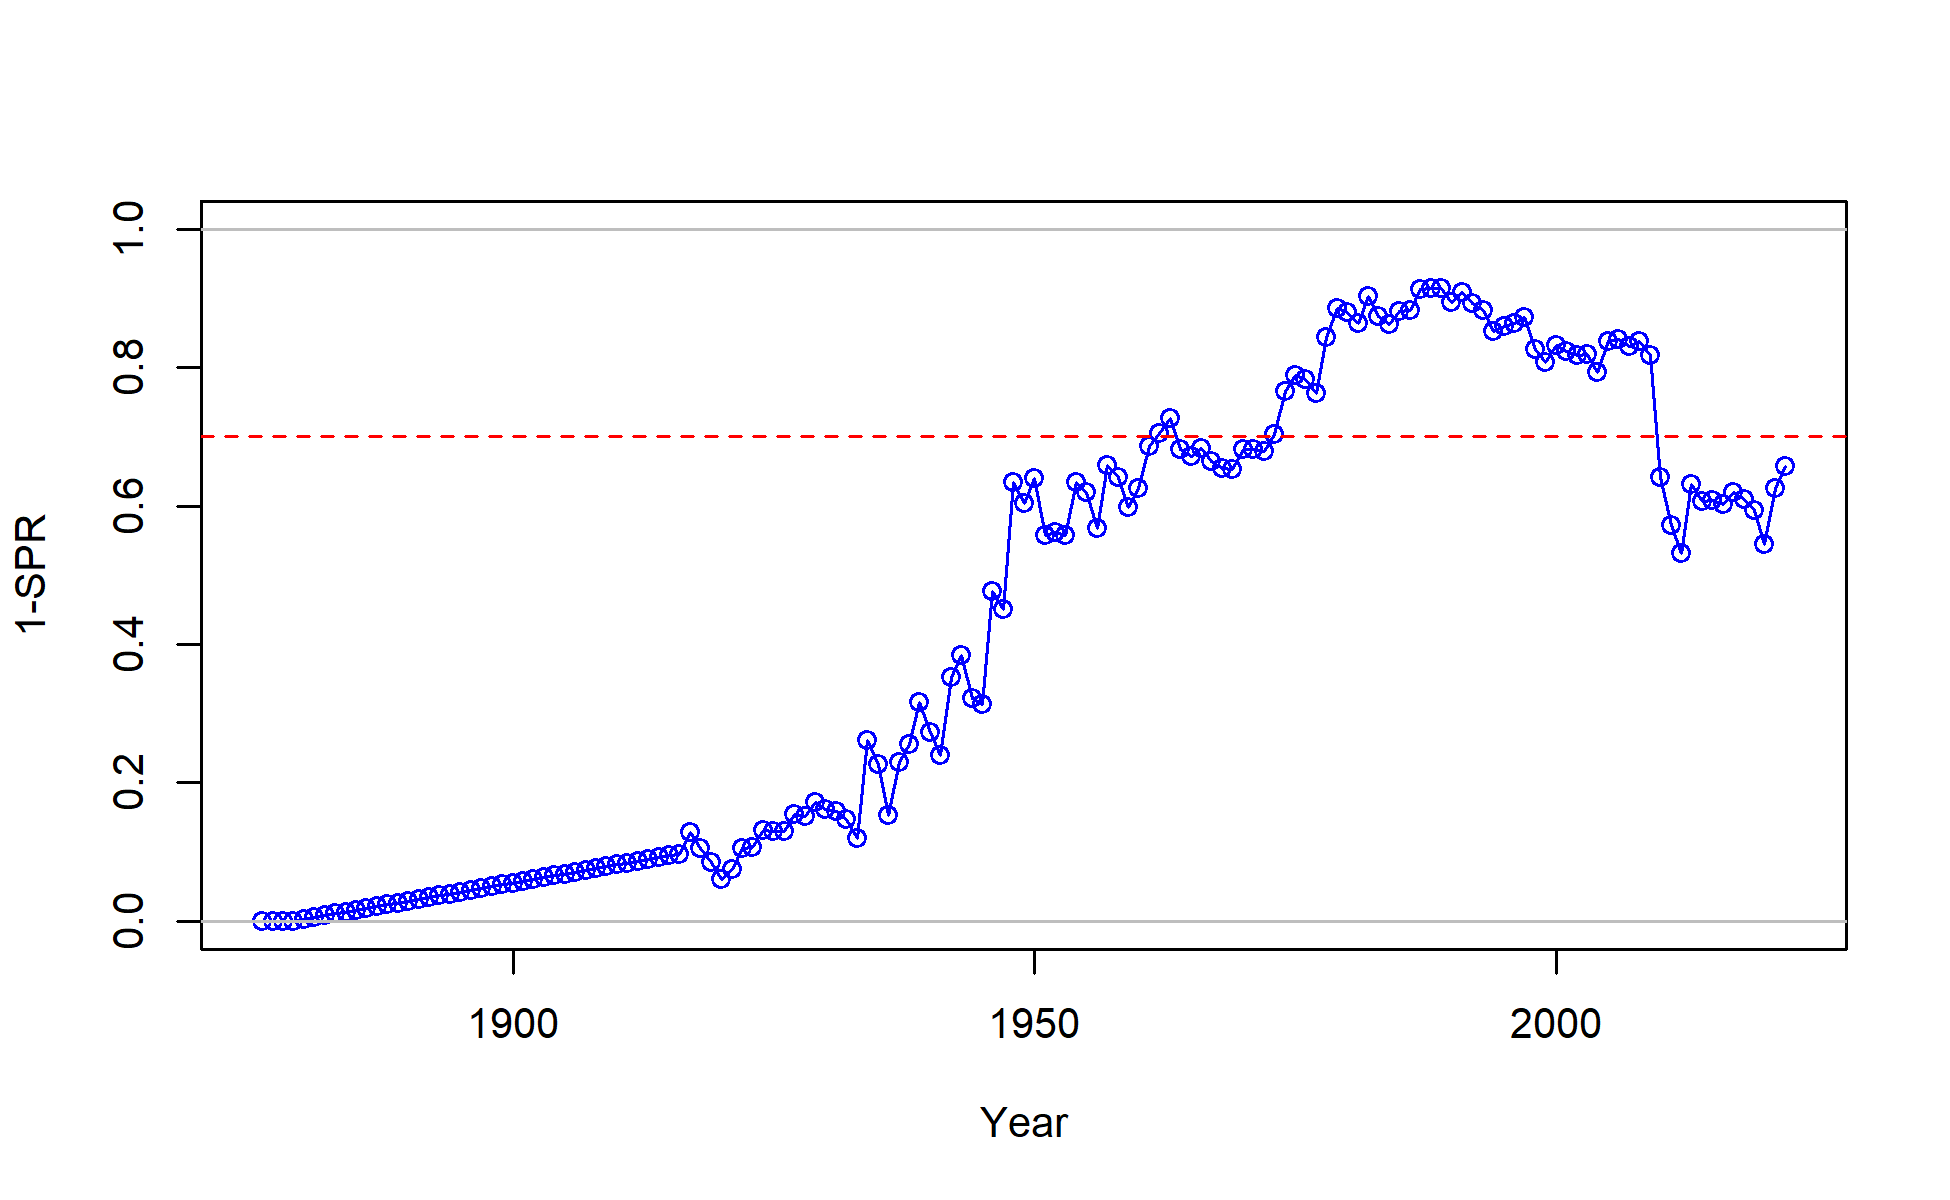
\includegraphics[width=1\textwidth,height=1\textheight]{../models/2023.005.001/plots/SPR2_minusSPRseries.png}
\caption{Estimated 1 - relative spawning ratio (SPR) by year for the base model. The management target is plotted as a red horizontal line and values above this reflect harvest in excess of the proxy harvest rate.\label{fig:es-1-spr}}
\end{figure}

\clearpage

\hypertarget{ecosystem-considerations}{%
\subsection*{Ecosystem considerations}\label{ecosystem-considerations}}
\addcontentsline{toc}{subsection}{Ecosystem considerations}

Replace text with a summary of reviewed environmental and ecosystem factors that appear to be correlated with stock dynamics. These may include variability in they physical environment, habitat, competitors, prey, or predators that directly or indirectly affects the stock's status, vital rates (growth, survival, productivity/recruitment) or range and distribution. Note which, if any, ecosystem factors are used in the assessment and how (e.g., as background information, in data preparations, as data inputs, in decisions about model structure).

\hypertarget{reference-points}\), i.e., the \(B_{MSY}\) proxy and the equilibrium stock size that results from fishing at the default harvest rate, i.e., the \(F_{MSY}\) proxy. Include Table of estimated reference points for ssb, SPR, exploitation rate, and yield based on SSB proxy for MSY, SPR proxy for MSY, and estimated MSY values.

\begin{figure}
\centering
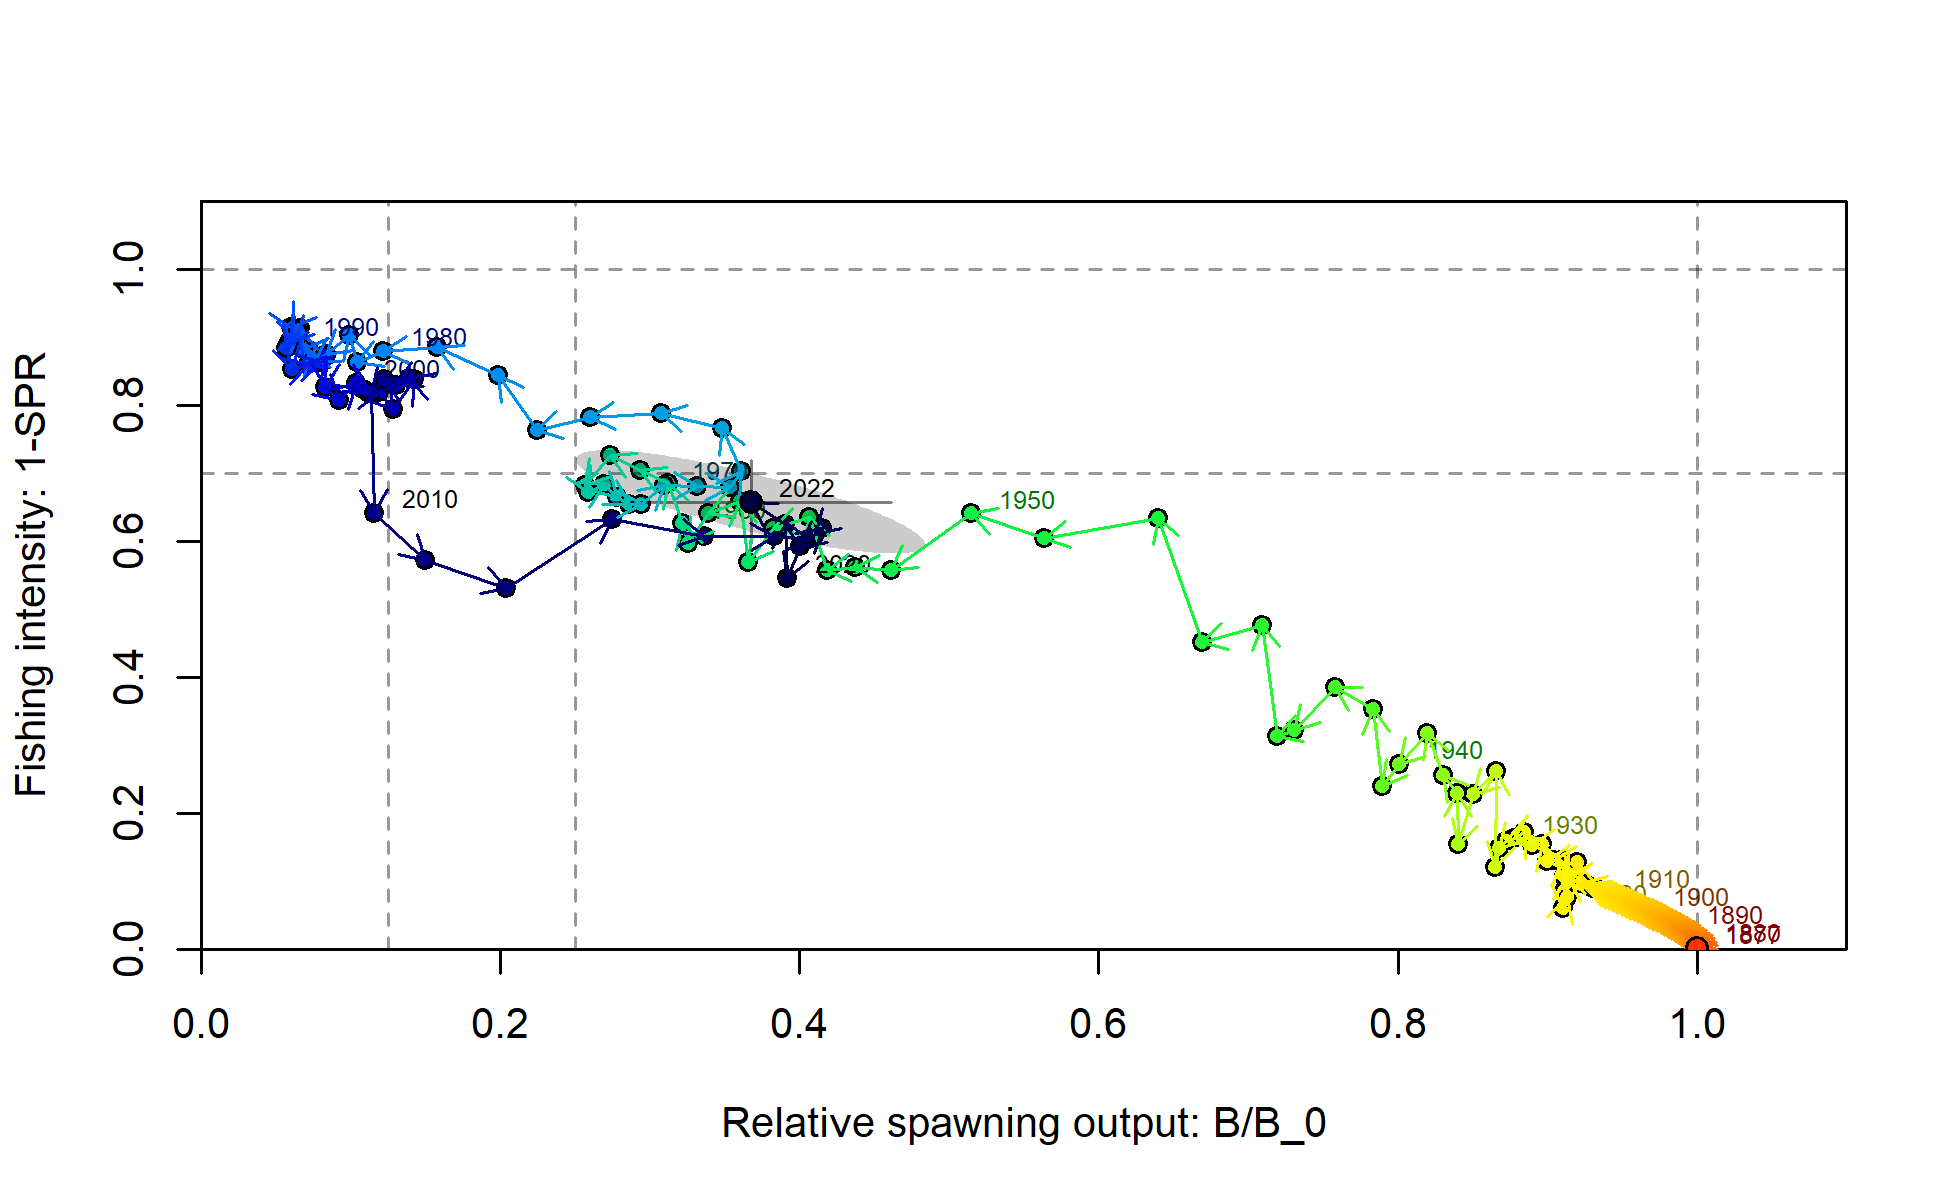
\includegraphics[width=1\textwidth,height=1\textheight]{../models/2023.005.001/plots/SPR4_phase.png}
\caption{Phase plot of estimated 1-SPR versus fraction unfished for the base model.\label{fig:es-phase}}
\end{figure}

\begin{figure}
\centering
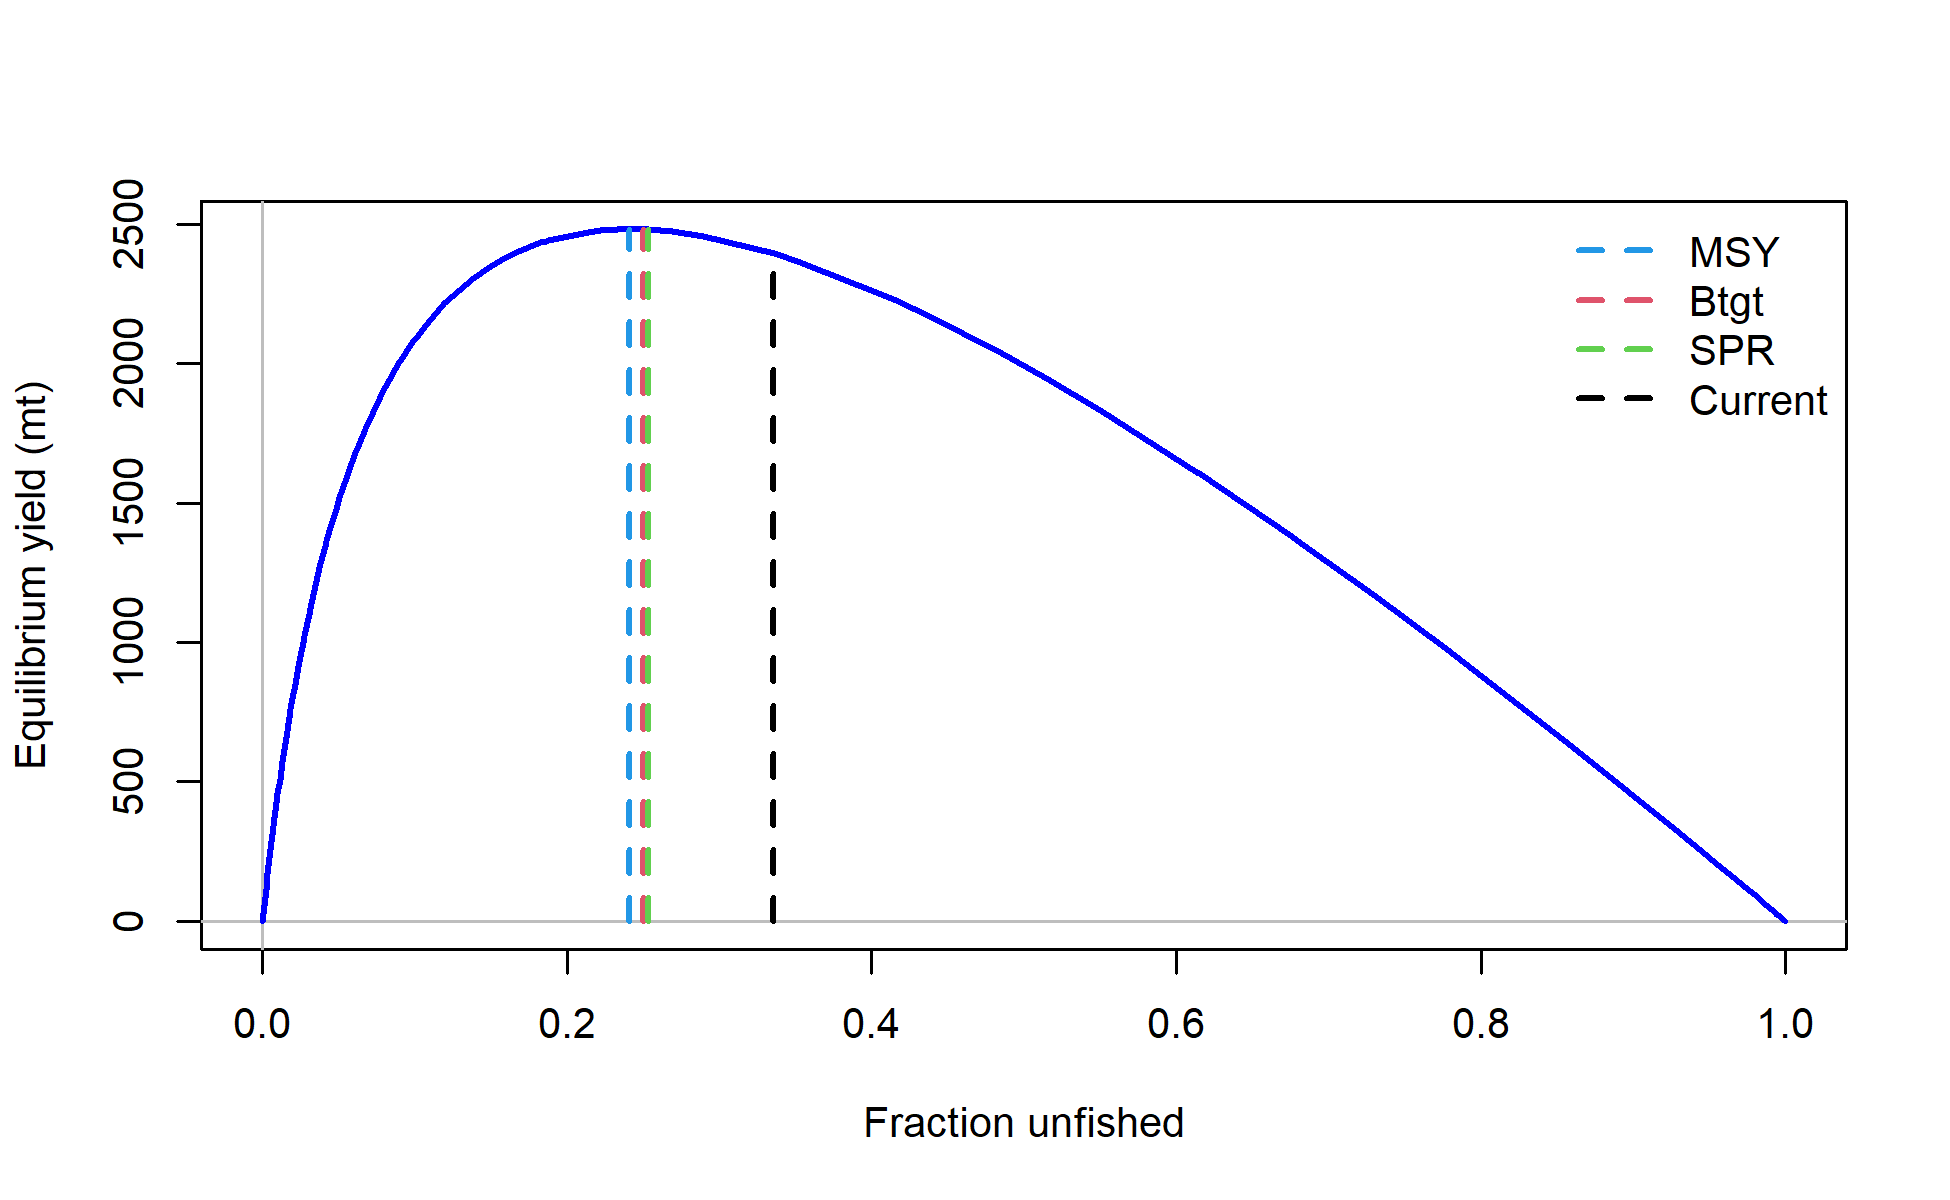
\includegraphics[width=1\textwidth,height=1\textheight]{../models/2023.005.001/plots/yield2_yield_curve_with_refpoints.png}
\caption{Equilibrium yield curve for the base case model. Values are based on the 2020 fishery selectivities and with steepness fixed at 0.80.\label{fig:es-yield}}
\end{figure}

\begingroup\fontsize{10}{12}\selectfont
\begingroup\fontsize{10}{12}\selectfont

\begin{longtable}[t]{r>{\centering\arraybackslash}p{2cm}>{\centering\arraybackslash}p{2cm}>{\centering\arraybackslash}p{2cm}}
\caption{\label{tab:referenceES}Summary of reference points and management quantities, including estimates of the  95 percent intervals.}\\
\toprule
 & Estimate & Lower Interval & Upper Interval\\
\midrule
\endfirsthead
\caption[]{Summary of reference points and management quantities, including estimates of the  95 percent intervals. \textit{(continued)}}\\
\toprule
 & Estimate & Lower Interval & Upper Interval\\
\midrule
\endhead

\endfoot
\bottomrule
\endlastfoot
Unfished Spawning Output & 22396.10 & 17650.48 & 27141.72\\
Unfished Age 3+ Biomass (mt) & 41559.40 & 34361.04 & 48757.76\\
Unfished Recruitment (R0) & 15477.80 & 11459.74 & 19495.86\\
Spawning Output (2023) & 7770.54 & 6437.66 & 9103.42\\
Fraction Unfished (2023) & 0.35 & 0.26 & 0.44\\
Reference Points Based SB25\textbackslash{}\% & NA & NA & NA\\
Proxy Spawning Output SB25\textbackslash{}\% & 5599.04 & 4412.63 & 6785.45\\
SPR Resulting in SB25\textbackslash{}\% & 0.30 & 0.30 & 0.30\\
Exploitation Rate Resulting in SB25\textbackslash{}\% & 0.18 & 0.16 & 0.20\\
Yield with SPR Based On SB25\textbackslash{}\% (mt) & 2484.25 & 2116.38 & 2852.12\\
Reference Points Based on SPR Proxy for MSY & NA & NA & NA\\
Proxy Spawning Output (SPR30) & 5673.69 & 4471.46 & 6875.92\\
SPR30 & 0.30 & NA & NA\\
Exploitation Rate Corresponding to SPR30 & 0.18 & 0.16 & 0.19\\
Yield with SPR30 at SB SPR (mt) & 2483.49 & 2115.78 & 2851.20\\
Reference Points Based on Estimated MSY Values & NA & NA & NA\\
Spawning Output at MSY (SB MSY) & 5414.88 & 4231.35 & 6598.41\\
SPR MSY & 0.29 & 0.28 & 0.30\\
Exploitation Rate Corresponding to SPR MSY & 0.18 & 0.16 & 0.20\\
MSY (mt) & 2485.04 & 2116.94 & 2853.14\\*
\end{longtable}
\endgroup{}
\endgroup{}


\clearpage

\hypertarget{management-performance}{%
\subsection*{Management performance}\label{management-performance}}
\addcontentsline{toc}{subsection}{Management performance}

Include Table of most recent 10 years of catches in comparison with OFL, ABC, HG, and OY/ACL values, overfishing levels, actual catch and discard. Include OFL (encountered), OFL (retained), and OFL (dead) if different due to discard and discard mortality.

\hypertarget{unresolved-problems-and-major-uncertainties}{%
\subsection*{Unresolved problems and major uncertainties}\label{unresolved-problems-and-major-uncertainties}}
\addcontentsline{toc}{subsection}{Unresolved problems and major uncertainties}

Replace text with any special issues that complicate scientific assessment, questions about the best model scenario, etc.

\hypertarget{decision-table-and-projections}{%
\subsection*{Decision table and projections}\label{decision-table-and-projections}}
\addcontentsline{toc}{subsection}{Decision table and projections}

Replace text with projected yields (OFL, ABC, and ACL), spawning biomass, and stock depletion levels for each year. OFL calculations should be based on the assumption that future catches equal ABCs and not OFLs.

\hypertarget{scientific-uncertainty}{%
\subsection*{Scientific uncertainty}\label{scientific-uncertainty}}
\addcontentsline{toc}{subsection}{Scientific uncertainty}

Replace text with the sigma value and the basis for its calculation.

\hypertarget{research-and-data-needs}{%
\subsection*{Research and data needs}\label{research-and-data-needs}}
\addcontentsline{toc}{subsection}{Research and data needs}

Replace text with information gaps that seriously impede the stock assessment.

\pagebreak
\setlength{\parskip}{5mm plus1mm minus1mm}
\pagenumbering{arabic}
\setcounter{page}{1}
\renewcommand{\thefigure}{\arabic{figure}}
\renewcommand{\thetable}{\arabic{table}}
\setcounter{table}{0}
\setcounter{figure}{0}

\hypertarget{introduction}{%
\section{Introduction}\label{introduction}}

This updated assessment does not attempt to reiterate all background information for petrale sole presented in the 2013 assessment document. Instead, only a few key assumptions are restated, along with a detailed description of changes made during the course of the update. Those interested in a more complete description of petrale sole life-history and the details of previous assessments should refer to the 2013 assessment (Haltuch, Ono, and Valero 2013).

\hypertarget{basic-information}{%
\subsection{Basic Information}\label{basic-information}}

Petrale Sole (\emph{Eopsetta jordani}) is a right-eyed flounder in the family Pleuronectidae ranging from the western Gulf of Alaska to the Coronado Islands, northern Baja California (Kramer et al. 1995; Love et al. 2005) with a preference for soft substrates at depths ranging from 0-550 m (Love et al. 2005). Common names include brill, California sole, Jordan's flounder, cape sole, round nose sole, English sole, soglia, petorau, nameta, and tsubame garei (Smith 1937; Gates and Frey 1974; Love 1996; Eschmeyer and Herald 1983). In northern and central California petrale sole are dominant on the middle and outer continental shelf. PacFIN fishery logbook data show that adults are caught in depths from 18 to 1,280 m off the U.S. West Coast with a majority of the catches of petrale sole being taken between 70-220 m during March through October, and between 290-440 m during November through February.

There is little information regarding the stock structure of petrale sole off the U.S. Pacific coast. No genetic research has been undertaken for petrale sole and there is no other published research indicating separate stocks of petrale sole within U.S. waters. Tagging studies show adult petrale sole can move up to 350 - 390 miles, having the ability to be highly migratory with the possibility for homing ability (Alverson and Chatwin 1957). Juveniles show little coast-wide or bathymetric movement while studies suggest that adults generally move inshore and northward onto the continental shelf during the spring and summer to feeding grounds and offshore and southward during the fall and winter to deep water spawning grounds (Horton 1989; Love 1996). Adult petrale sole can tolerate a wide range of bottom temperatures (Perry, Stocker, and Fargo 1994).

Tagging studies indicate some mixing of adults between different spawning groups. DiDonato and Pasquale (1970) reported that five fish tagged on the Willapa Deep grounds during the spawning season were recaptured during subsequent spawning seasons at other deepwater spawning grounds, as far south as Eureka (northern California) and the Umpqua River (southern Oregon). However, Pedersen (1975) reported that most of the fish (97\%) recaptured from spawning grounds in winter were originally caught and tagged on those same grounds.

Mixing of fish from multiple deep water spawning grounds likely occurs during the spring and summer when petrale sole are feeding on the continental shelf. Fish that were captured, tagged, and released off the northwest Coast of Washington during May and September were subsequently recaptured during winter from spawning grounds off Vancouver Island (British Columbia, 1 fish), Heceta Bank (central Oregon, 2 fish), Eureka (northern California, 2 fish), and Halfmoon Bay (central California, 2 fish) (Pederson, 1975). Fish tagged south of Fort Bragg (central California) during July 1964 were later recaptured off Oregon (11 fish), Washington (6 fish), and Swiftsure Bank (southwestern tip of Vancouver Island, 1 fish) (D. Thomas, California Department of Fish and Game, Menlo Park, CA, cited by Sampson and Lee (1999)).

The highest densities of spawning adults off of British Columbia, as well as of eggs, larvae and juveniles, are found in the waters around Vancouver Island. Adults may utilize nearshore areas as summer feeding grounds and non-migrating adults may stay there during winter (P. J. Starr and Fargo 2004).

Past assessments completed by Demory (1984,), Turnock et al. (1993), and Sampson and Lee (1999) considered petrale sole in the Columbia and U.S.-Vancouver INPFC areas a single stock. Sampson and Lee (1999) assumed that petrale sole in the Eureka and Monterey INPFC areas represented two additional distinct socks. The 2005 petrale sole assessment assumed two stocks, northern (U.S.-Vancouver and Columbia INPFC areas) and southern (Eureka, Monterey and Conception INPFC areas), to maintain continuity with previous assessments. Three stocks (West Coast Vancouver Island, Queen Charlotte Sound, and Heceta Strait) are considered for petrale sole in the waters off British Columbia, Canada (P. J. Starr and Fargo 2004). The 2009, 2011, 2013, and 2015 assessments integrate the previously separate north-south assessments to provide a coast-wide status evaluation. The decision to conduct a single-area assessment is based on strong evidence of a mixed stock from tagging studies, a lack of genetic studies on stock structure, and a lack of evidence for differences in growth between the 2005 northern and southern assessment areas and from examination of the fishery size-at-age data, as well as confounding differences in data collection between Washington, Oregon, and California. This 2019 update assessment provides a coast-wide status evaluation for petrale sole using data through 2018.

Fishing fleets are separated both geographically and seasonally to account for spatial and seasonal patterns in catch given the coast-wide assessment area. The petrale sole fisheries possess a distinct seasonality, with catches peaking during the winter months, so the fisheries are divided into winter (November-February) and summer (March-October) fisheries. Note that the ``fishing year'' for this assessment (November 1 to October 31) differs from the standard calendar year. The U.S.-Canadian border is the northern boundary for the assessed stock, although the basis for this choice is due to political and current management needs rather than the population dynamics. Given the lack of clear information regarding the status of distinct biological populations, this assessment treats the U.S. Petrale Sole resource from the Mexican border to the Canadian border as a single coast-wide stock.

\hypertarget{life-history}{%
\subsection{Life History}\label{life-history}}

Petrale Sole spawn during the winter at several discrete deepwater sites (270-460 m) off the U.S. West Coast, from November to April, with peak spawning taking place from December to February (Harry 1956; Best 1960; Gregory and Jow 1976; Castillo, Li, and Golden 1993; Reilly et al. 1994; Castillo 1995; Love 1996). Females spawn once each year and fecundity varies with fish size, with one large female laying as many as 1.5 million eggs (Porter 1964). Petrale Sole eggs are planktonic, ranging in size from 1.2 to 1.3 mm, and are found in deep water habitats at water temperatures of 4-10 degrees C and salinities of 25-30 ppt (Best 1960; Ketchen and Forrester 1966; Alderdice and Forrest 1971; Gregory and Jow 1976). The duration of the egg stage can range from approximately 6 to 14 days (Alderdice and Forrest 1971; Love 1996). The most favorable conditions for egg incubation and larval growth are 6-7 degrees C and 27.5-29.5 ppt (Ketchen and Forrester 1966; Alderdice and Forrest 1971).

Petrale Sole spawn during the winter at several discrete deepwater sites (270-460 m) off the U.S. West Coast, from November to April, with peak spawning taking place from December to February (Harry 1959; Best 1960; Gregory and Jow 1976; Castillo, Li, and Golden 1993; Reilly et al. 1994; Love 1996). Females spawn once each year and fecundity varies with fish size, with one large female laying as many as 1.5 million eggs (Porter 1964). Petrale Sole eggs are planktonic, ranging in size from 1.2 to 1.3 mm, and are found in deep water habitats at water temperatures of 4-10 degrees C and salinities of 25-30 ppt (Best 1960; Ketchen and Forrester 1966; Alderdice and Forrest 1971; Gregory and Jow 1976). The duration of the egg stage can range from approximately 6 to 14 days (Alderdice and Forrest 1971; Love 1996). The most favorable conditions for egg incubation and larval growth are 6-7 degrees C and 27.5-29.5 ppt (Ketchen and Forrester 1966; Alderdice and Forrest 1971; Castillo 1995).

Adult petrale sole achieve a maximum size of around 50 cm and 63 cm for males and females, respectively (Best 1963; Pedersen 1975). The maximum length reported for petrale sole is 70 cm (Eschmeyer and Herald 1983; Love et al. 2005) while the maximum observed break-and-burn age is 31 years (Haltuch, Ono, and Valero 2013).

\hypertarget{ecosystem-considerations-1}{%
\subsection{Ecosystem Considerations}\label{ecosystem-considerations-1}}

Petrale Sole juveniles are carnivorous, foraging on annelid worms, clams, brittle star, mysids, sculpin, amphipods, and other juvenile flatfish (Casilla et al. 1998; Pearsall and Fargo 2007). Predators on juvenile petrale sole include adult petrale sole as well as other larger fish (Casilla et al. 1998) while adults are preyed upon by marine mammals, sharks, and larger fishes (Trumble 1995; Love 1996; Casilla et al. 1998).

One of the ambushing flatfishes, adult petrale sole have diverse diets that become more piscivorous at larger sizes (Allen, Pondella, and Horn 2006). Adult petrale sole are found on sandy and sand-mud bottoms (Eschmeyer and Herald 1983) foraging for a variety of invertebrates including, crab, octopi, squid, euphausiids, and shrimp, as well as anchovies. hake, herring, sand lance, and other smaller rockfish and flatfish (Kravitz, Pearcy, and Guin 1977; Birtwell, Wood, and Gordon 1984; Reilly et al. 1994; Love 1996; Pearsall and Fargo 2007). In Canadian waters evidence suggests that petrale sole tend to prefer herring (Pearsall and Fargo 2007). On the continental shelf petrale sole generally co-occur with English sole, rex sole, Pacific sanddab, and rock sole (Kravitz, Pearcy, and Guin 1977).

Ecosystem factors have not been explicitly modeled in this assessment, but there are several aspects of the California current ecosystem that may impact petrale sole population dynamics and warrant further research. Castillo (1992) and Castillo et al. (1995) suggest that density-independent survival of early life stages is low and show that offshore Ekman transportation of eggs and larvae may be an important source of variation in year-class strength in the Columbia INPFC area. The effects of the Pacific Decadal Oscillation (PDO) on California current temperature and productivity (Mantua et al. 1997) may also contribute to non-stationary recruitment dynamics for petrale sole. The prevalence of a strong late 1990s year-class for many West Coast groundfish species suggests that environmentally driven recruitment variation may be correlated among species with relatively diverse life history strategies. Although current research efforts along these lines are limited, a more explicit exploration of ecosystem processes may be possible in future petrale sole stock assessments.

\hypertarget{historical-and-current-fishery-information}{%
\subsection{Historical and Current Fishery Information}\label{historical-and-current-fishery-information}}

Petrale Sole have been caught in the flatfish fishery off the U.S. Pacific coast since the late 19th century. The fishery first developed off of California where, prior to 1876, fishing in San Francisco Bay was by hand or set lines and beach seining (Scofield 1948). By 1880 two San Francisco based trawler companies were running a total of six boats, extending the fishing grounds beyond the Golden Gate Bridge northward to Point Reyes (Scofield 1948). Steam trawlers entered the fishery during 1888 and 1889, and four steam tugs based out of San Francisco were sufficient to flood market with flatfish (Scofield 1948). By 1915 San Francisco and Santa Cruz trawlers were operating at depths of about 45-100 m with catches averaging 10,000 lbs per tow or 3,000 lbs per hour (Scofield 1948). Flatfish comprised approximately 90\% of the catch with 20-25\% being discarded as unmarketable (Scofield 1948). During 1915 laws were enacted that prohibited dragging in California waters and making it illegal to possess a trawl net from Santa Barbara County southward (Scofield 1948). By 1934 twenty 56-72 foot diesel engine trawlers operated out of San Francisco fishing between about 55 and 185 m (Scofield 1948). From 1944-1947 the number of California trawlers fluctuated between 16 and 46 boats (Scofield 1948). Although the flatfish fishery in California was well developed by the 1950s and 1960s, catch statistics were not reported until 1970 (Heimann and Carlisle 1970). In this early California report petrale sole landings during 1916 to 1930 were not separated from the total flatfish landings.

The earliest trawl fishing off Oregon began during 1884-1885, and the fishery was solidly established by 1937, with the fishery increasing rapidly during WWII (Harry and Morgan, 1961). Initially trawlers stayed close to the fishing grounds adjacent to Newport and Astoria, operating at about 35-90 m between Stonewall Bank and Depoe Bay. Fishing operations gradually extended into deep water. For example, Newport-based trawlers were commonly fishing at about 185 m in 1949, at about 185-365 m by 1952, and at about 550 m by 1953.

Alverson and Chatwin (1957) describe the history of the petrale sole fishery off of Washington and British Columbia with fishing grounds ranging from Cape Flattery to Destruction Island. Petrale Sole catches off of Washington were small until the late 1930s with the fishery extending to about 365 m following the development of deepwater rockfish fisheries during the 1950s.

By the 1950s the petrale sole fishery was showing signs of depletion with reports suggesting that petrale sole abundance had declined by at least 50\% from 1942 to 1947 (Harry 1956). Sampson and Lee (1999) reported that three fishery regulations were implemented during 1957-67: 1) a winter closure off Oregon, Washington and British Columbia, 2) a 3,000 lb per trip limit, and 3) no more than two trips per month during 1957. With the 1977 enactment of the Magnuson Fishery Conservation and Management Act (MFCMA) the large foreign-dominated fishery that had developed since the late 1960s was replaced by the domestic fishery that continues today. Petrale Sole are harvested almost exclusively by bottom trawls in the U.S. West Coast groundfish fishery. Recent petrale sole catches exhibit marked seasonal variation, with substantial portions of the annual harvest taken from the spawning grounds during December and January. Evidence suggests that the winter fishery on the deepwater spawning grounds developed sporadically during the 1950s and 1960s as fishers discovered new locations (e.g., Alverson and Chatwin (1957); Ketchen and Forrester (1966)). Both historical and current petrale sole fisheries have primarily relied upon trawl fleets. Fishery removals were divided among 4 fleets: 1) winter North trawl, 2) summer North trawl, 3) winter South trawl, and 4) summer South trawl. Landings for the North fleet are defined as fish landed in Washington and Oregon ports. Landings for the South fleet are defined as fish landed in California ports.

\hypertarget{summary-of-management-history-and-performance}{%
\subsection{Summary of Management History and Performance}\label{summary-of-management-history-and-performance}}

Beginning in 1983 the Pacific Fishery Management Council (PFMC) established coast-wide annual catch limits (ACLs) for the annual harvests of petrale sole in the waters off the U.S. West Coast. The first assessment of West Coast petrale sole occurred in 1984 (Demory 1984). Based on the 1999 assessment a coast-wide ACL of 2,762 mt was specified and remained unchanged between 2001 and 2006.

The 2005 assessment of petrale sole stock assessment split the stock into two areas, the northern area that included U.S.-Vancouver and Columbia INPFC areas and the southern area that included the Eureka, Monterey and Conception INPFC areas (Lai et al. 2005). While petrale sole stock structure is not well understood, CPUE and geographical differences between states were used to support the use of two separate assessment areas. In 2005 petrale sole were estimated to be at 34 and 29\% of unfished spawning stock biomass in the northern and southern areas, respectively. In spite of different models and data, the biomass trends were qualitatively similar in both areas, providing support for a coast-wide stock. This assessment estimated that petrale sole had historically been below the Pacific Council's minimum stock size threshold of 25\% of unfished biomass from the mid-1970s until just prior to the completion of the assessment, with estimated harvest rates in excess of the target fishing mortality rate implemented for petrale sole at that time (F40\%). However, the 2005 stock assessment determined that the stock was in the precautionary zone and was not overfished (i.e., the spawning stock biomass was not below 25\% of the unfished spawning stock biomass). Based on the 2005 stock assessment results, ACLs were set at 3,025 mt and 2,919 mt for 2007 and 2008, respectively, with an ACT of 2,499 mt for both years.

In comparison to the 1999 assessment of petrale sole, the 2005 assessment represented a significant change in the perception of petrale sole stock status. The stock assessment conducted in 1999 (Washington-Oregon only) estimated the spawning stock biomass in 1998 at 39\% of unfished stock biomass. Although the estimates of 1998 spawning-stock biomass were little changed between the 1999 and 2005 (Northern area) assessments, the estimated depletion in the 2005 assessment was much lower. The change in status between the 1999 and 2005 analyses was due to the introduction of a reconstructed catch history in 2005, which spanned the entire period of removals. The 1999 stock assessment used a catch history that started in 1977, after the bulk of the removals from the fishery had already taken place. Thus the 1999 stock assessment produced a more optimistic view of the petrale stock's level of depletion. The stock's estimated decline in status between the 2005 and 2009 assessments was driven primarily by a significant decline in the trawl-survey index over that period. The 2011 assessment concluded that the stock status continued to be below the target of 25\% of unfished biomass.

The 2009 coast-wide stock assessment estimated that the petrale sole stock had declined from its 2005 high to 11.6\% of the unfished spawning stock biomass (Haltuch and Hicks 2009). The petrale sole was declared overfished based on newly adopted management targets (e.g., target spawning biomass for flatfish stocks defined as 25\% and overfished threshold of 12.5\% of unfished spawning stock biomass) resulting in a rebuilding plan and catch restrictions for petrale sole. The stock was declared rebuilt based on the results of the 2015 update stock assessment which estimated the coastwide biomass at 30.7\% of unfished spawning stock output with ACLs of 3,136 and 3,013 in 2017 and 2018 respectively (Stawitz et al. 2015).

For additional information on changes in the petrale sole fishery please see the 2013 stock assessment (Haltuch, Ono, and Valero 2013).

\hypertarget{fisheries-off-canada-and-alaska}{%
\subsection{Fisheries off Canada and Alaska}\label{fisheries-off-canada-and-alaska}}

The Canadian fishery developed rapidly during the late 1940s to mid-1950s following the discovery of petrale sole spawning aggregations off the West Coast of Vancouver Island (Anon 2001). Annual landings of petrale sole in British Columbia peaked at 4,800 mt in 1948 but declined significantly after the mid-1960s (Anon 2001). By the 1970s, analysis conducted by Pederson (1975) suggested that petrale sole abundance was low and abundance remained low into the 1990s. In the early 1990s vessel trip quotas were established to try to halt the decline in petrale sole abundance (Anon 2001). Winter quarter landings of petrale sole were limited to 44,000 lb per trip during 1985-91; to 10,000 lb per trip during 1991-95; and to 2,000 lb per trip in 1996. Biological data collected during 1980-1996 showed a prolonged decline in the proportion of young fish entering the population (Anon 2001). Therefore, no directed fishing for petrale sole has been permitted in Canada since 1996 due to a continuing decline in long term abundance (Fargo 1997; Anon 2001). As of 2005 petrale sole off of British Columbia were treated as three ``stocks'' and were still considered to be at low levels. The recent assessments for the Canadian stocks have been based on catch histories and limited biological data.

In Alaska petrale sole are not targeted in the Bering Sea/Aleutian Island fisheries and are managed as a minor species in the ``Other Flatfish'' stock complex.

\hypertarget{data}{%
\section{Data}\label{data}}

Data comprise the foundational components of stock assessment models. The decision to include or exclude particular data sources in an assessment model depends on many factors. These factors often include, but are not limited to, the way in which data were collected (e.g., measurement method and consistency); the spatial and temporal coverage of the data; the quantity of data available per desired sampling unit; the representativeness of the data to inform the modeled processes of importance; timing of when the data were provided; limitations imposed by the Terms of Reference; and the presence of an avenue for the inclusion of the data in the assessment model. Attributes associated with a data source can change through time, as can the applicability of the data source when different modeling approaches are explored (e.g., stock structure or time-varying processes). Therefore, the specific data sources included or excluded from this assessment should not necessarily constrain the selection of data sources applicable to future stock assessments for petrale sole. Even if a data source is not directly used in the stock assessment they can provide valuable insights into biology, fishery behavior, or localized dynamics.

Data from a wide range of programs were available for possible inclusion in the current assessment model. Descriptions of each data source included in the model (Figure \ref{fig:data-plot}) and sources that were explored but not included in the base model are provided below. Data that were excluded from the base model were explicitly explored during the development of this stock assessment or have not changed since their past exploration in a previous petrale sole stock assessment. In some cases, the inclusion of excluded data sources were explored through sensitivity analyses (see Section \ref{assessment-model}).

\hypertarget{fishery-dependent-data}{%
\subsection{Fishery-Dependent Data}\label{fishery-dependent-data}}

Fishery removals were divided among 4 fleets: 1) winter North trawl, 2) summer North trawl, 3) winter South trawl, and 4) summer South trawl. Landings for the North fleet are defined as fish landed in Washington and Oregon ports. Landings for the South feet are defined as fish landed in California ports. The landings of petrale sole by gear types other than groundfish-trawl have been inconsequential, averaging less than 2.5\% of the coast-wide landings. The non-trawl landings (that consist of only a small fraction of the total landings) are included in the trawl landings.

\hypertarget{fishery-independent-data}{%
\subsection{Fishery-Independent Data}\label{fishery-independent-data}}

\hypertarget{section}{%
\subsubsection{\texorpdfstring{\acrlong{s-aslope}}{}}\label{section}}

The \gls{s-aslope} operated during the months of October to November aboard the R/V \emph{Miller Freeman}. Partial survey coverage of the US west coast occurred during the years 1988-1996 and complete coverage (north of 34\textdegree 30\textquotesingle S) during the years 1997 and 1999-2001. Typically, only these four years that are seen as complete surveys are included in assessments.

\hypertarget{section-1}{%
\subsubsection{\texorpdfstring{\acrlong{s-ccfrp}}{}}\label{section-1}}

Since 2007, the \gls{s-ccfrp} has monitored several areas in California to evaluate the performance of \glspl{mpa} and understand nearshore fish populations (Wendt and Starr 2009; R. M. Starr et al. 2015). In 2017, the survey expanded beyond the four \Gls{mpa}s in central California (Año Nuevo, Point Lobos, Point Buchon, and Piedras Blancas) to include the entire California coast. Fish are collected by volunteer anglers aboard \glspl{cpfv} guided by one of the following academic institutions based on proximity to fishing location: Humboldt State University; Bodega Marine Laboratories; Moss Landing Marine Laboratories; Cal Poly San Luis Obispo; University of California, Santa Barbara; and Scripps Institution of Oceanography.

Surveys consist of fishing with hook-and-line gear for 30-45 minutes within randomly chosen 500 by 500 m grid cells within and outside \glspl{mpa}. Prior to 2017, all fish were measured for length and release or descended to depth; since then, some were sampled for otoliths and fin clips.

\hypertarget{section-2}{%
\subsubsection{\texorpdfstring{\acrlong{s-tri}}{}}\label{section-2}}

The \gls{s-tri} was first conducted by the \gls{afsc} in 1977, and the survey continued until 2004 (Weinberg et al. 2002). Its basic design was a series of equally-spaced east-to-west transects across the continential shelf from which searches for tows in a specific depth range were initiated. The survey design changed slightly over time. In general, all of the surveys were conducted in the mid summer through early fall. The 1977 survey was conducted from early July through late September. The surveys from 1980 through 1989 were conducted from mid-July to late September. The 1992 survey was conducted from mid July through early October. The 1995 survey was conducted from early June through late August. The 1998 survey was conducted from early June through early August. Finally, the 2001 and 2004 surveys were conducted from May to July.

Haul depths ranged from 91-457 m during the 1977 survey with no hauls shallower than 91 m. Due to haul performance issues and truncated sampling with respect to depth, the data from 1977 were omitted from this analysis. The surveys in 1980, 1983, and 1986 covered the US West Coast south to 36.8\textdegree N latitude and a depth range of 55-366 m. The surveys in 1989 and 1992 covered the same depth range but extended the southern range to 34.5\textdegree N (near Point Conception). From 1995 through 2004, the surveys covered the depth range 55-500 m and surveyed south to 34.5\textdegree N. In 2004, the final year of the \gls{s-tri} series, the \gls{nwfsc} \gls{fram} conducted the survey following similar protocols to earlier years.

\hypertarget{section-3}{%
\subsubsection{\texorpdfstring{\acrlong{s-wcgbt}}{}}\label{section-3}}

The \Gls{s-wcgbt} is based on a random-grid design; covering the coastal waters from a depth of 55-1,280 m (Bradburn, Keller, and Horness 2011). This design generally uses four industry-chartered vessels per year assigned to a roughly equal number of randomly selected grid cells and divided into two `passes' of the coast. Two vessels fish from north to south during each pass between late May to early October. This design therefore incorporates both vessel-to-vessel differences in catchability, as well as variance associated with selecting a relatively small number (approximately 700) of possible cells from a very large set of possible cells spread from the Mexican to the Canadian borders.

\hypertarget{biological-data}{%
\subsection{Biological Data}\label{biological-data}}

\hypertarget{natural-mortality}{%
\subsubsection{Natural Mortality}\label{natural-mortality}}

\hypertarget{maturation-and-fecundity}{%
\subsubsection{Maturation and Fecundity}\label{maturation-and-fecundity}}

\hypertarget{sex-ratio}{%
\subsubsection{Sex Ratio}\label{sex-ratio}}

\hypertarget{length-weight-relationship}{%
\subsubsection{Length-Weight Relationship}\label{length-weight-relationship}}

\hypertarget{growth-length-at-age}{%
\subsubsection{Growth (Length-at-Age)}\label{growth-length-at-age}}

\hypertarget{ageing-precision-and-bias}{%
\subsubsection{Ageing Precision and Bias}\label{ageing-precision-and-bias}}

\hypertarget{environmental-and-ecosystem-data}{%
\subsection{Environmental and Ecosystem Data}\label{environmental-and-ecosystem-data}}

\hypertarget{assessment-model}{%
\section{Assessment Model}\label{assessment-model}}

\hypertarget{summary-of-previous-assessments-and-reviews}{%
\subsection{Summary of Previous Assessments and Reviews}\label{summary-of-previous-assessments-and-reviews}}

\hypertarget{history-of-modeling-approaches-not-required-for-an-update-assessment}{%
\subsubsection{History of Modeling Approaches (not required for an update assessment)}\label{history-of-modeling-approaches-not-required-for-an-update-assessment}}

\hypertarget{most-recent-star-panel-and-ssc-recommendations-not-required-for-an-update-assessment}{%
\subsubsection{Most Recent STAR Panel and SSC Recommendations (not required for an update assessment)}\label{most-recent-star-panel-and-ssc-recommendations-not-required-for-an-update-assessment}}

\hypertarget{response-to-groundfish-subcommittee-requests-not-required-in-draft}{%
\subsubsection{Response to Groundfish Subcommittee Requests (not required in draft)}\label{response-to-groundfish-subcommittee-requests-not-required-in-draft}}

\hypertarget{model-structure-and-assumptions}{%
\subsection{Model Structure and Assumptions}\label{model-structure-and-assumptions}}

\hypertarget{model-changes-from-the-last-assessment-not-required-for-an-update-assessment}{%
\subsubsection{Model Changes from the Last Assessment (not required for an update assessment)}\label{model-changes-from-the-last-assessment-not-required-for-an-update-assessment}}

\hypertarget{modeling-platform-and-structure}{%
\subsubsection{Modeling Platform and Structure}\label{modeling-platform-and-structure}}

General model specifications (e.g., executable version, model structure, definition of fleets and areas)

\hypertarget{model-parameters}{%
\subsubsection{Model Parameters}\label{model-parameters}}

Describe estimated vs.~fixed parameters, priors

\hypertarget{key-assumptions-and-structural-choices}{%
\subsubsection{Key Assumptions and Structural Choices}\label{key-assumptions-and-structural-choices}}

\hypertarget{base-model-results}{%
\subsection{Base Model Results}\label{base-model-results}}

\hypertarget{parameter-estimates}{%
\subsubsection{Parameter Estimates}\label{parameter-estimates}}

\hypertarget{fits-to-the-data}{%
\subsubsection{Fits to the Data}\label{fits-to-the-data}}

\hypertarget{population-trajectory}{%
\subsubsection{Population Trajectory}\label{population-trajectory}}

\hypertarget{reference-points-1}{%
\subsubsection{Reference Points}\label{reference-points-1}}

\hypertarget{model-diagnostics}{%
\subsection{Model Diagnostics}\label{model-diagnostics}}

Describe all diagnostics

\hypertarget{convergence}{%
\subsubsection{Convergence}\label{convergence}}

\hypertarget{sensitivity-analyses}{%
\subsubsection{Sensitivity Analyses}\label{sensitivity-analyses}}

\hypertarget{retrospective-analysis}{%
\subsubsection{Retrospective Analysis}\label{retrospective-analysis}}

\hypertarget{likelihood-profiles}{%
\subsubsection{Likelihood Profiles}\label{likelihood-profiles}}

\hypertarget{unresolved-problems-and-major-uncertainties-1}{%
\subsubsection{Unresolved Problems and Major Uncertainties}\label{unresolved-problems-and-major-uncertainties-1}}

\hypertarget{management}{%
\section{Management}\label{management}}

\hypertarget{reference-points-2}{%
\subsection{Reference Points}\label{reference-points-2}}

\hypertarget{unresolved-problems-and-major-uncertainties-2}{%
\subsection{Unresolved Problems and Major Uncertainties}\label{unresolved-problems-and-major-uncertainties-2}}

\hypertarget{harvest-projections-and-decision-tables}{%
\subsection{Harvest Projections and Decision Tables}\label{harvest-projections-and-decision-tables}}

\hypertarget{evaluation-of-scientific-uncertainty}{%
\subsection{Evaluation of Scientific Uncertainty}\label{evaluation-of-scientific-uncertainty}}

\hypertarget{research-and-data-needs-1}{%
\subsection{Research and Data Needs}\label{research-and-data-needs-1}}

\hypertarget{acknowledgments}{%
\section{Acknowledgments}\label{acknowledgments}}

Here are all the mad props!

\clearpage

\hypertarget{references}{%
\section{References}\label{references}}

\hypertarget{refs}{}
\begin{CSLReferences}{1}{0}
\leavevmode\vadjust pre{\hypertarget{ref-alderdice_effects_1971}{}}%
Alderdice, D. F., and C. R. Forrest. 1971. {``Effects of Salinity and Temperature on Embryonic Development of the Petrale Sole(\emph{{Eopsetta} Jordani}).''} \emph{Journal of Fisheries Research Board Canada} 28: 727--44.

\leavevmode\vadjust pre{\hypertarget{ref-allen_ecology_2006}{}}%
Allen, Larry G., Daniel J. Pondella, and M. H. Horn. 2006. \emph{The Ecology of Marine Fishes: {California} and Adjacent Waters}. Los Angeles: University of California Press.

\leavevmode\vadjust pre{\hypertarget{ref-alverson_results_1957}{}}%
Alverson, D. L., and B. M. Chatwin. 1957. {``Results from Tagging Experiments on a Spawning Stock of Petrale Sole, \emph{{Eopsetta} Jordani} ({Lockington}).''} \emph{Journal of Fisheries Research Board Canada} 14: 953--74.

\leavevmode\vadjust pre{\hypertarget{ref-anon_fish_2001}{}}%
Anon. 2001. \emph{Fish Stocks of the {Pacific} Coast}. Cat No. Fs23-397/2001E. Fisheries; Oceans Canada.

\leavevmode\vadjust pre{\hypertarget{ref-best_petrale_1960}{}}%
Best, E. A. 1960. {``Petrale {Sole}. {In}: {California} Ocean Fisheries Resources to the Year 1960.''} California Department of Fish; Game.

\leavevmode\vadjust pre{\hypertarget{ref-best_e.a._movements_1963}{}}%
---------. 1963. {``Movements of Petrale Sole, \emph{{Eopsetta} Jordani}, Tagged Off of {California}.''} \emph{Pacific Marine Fisheries Commission Bulletin} 6: 24--38.

\leavevmode\vadjust pre{\hypertarget{ref-birtwell_fish_1984}{}}%
Birtwell, I. K., M. Wood, and D. K. Gordon. 1984. {``Fish Diets and Benthic Invertebrates in the Estuary of the {Somass} {River}, {Port} {Alberni}, {British} {Columbia}.''} 1799. California Manuscript Report of Fisheries; Aquatic Sciences.

\leavevmode\vadjust pre{\hypertarget{ref-bradburn_2003_2011}{}}%
Bradburn, M. J., A. A Keller, and B. H. Horness. 2011. {``The 2003 to 2008 {US} {West} {Coast} Bottom Trawl Surveys of Groundfish Resources Off {Washington}, {Oregon}, and {California}: Estimates of Distribution, Abundance, Length, and Age Composition.''} US Department of Commerce, National Oceanic; Atmospheric Administration, National Marine Fisheries Service.

\leavevmode\vadjust pre{\hypertarget{ref-casilla_essential_1998}{}}%
Casilla, E., L. Crockett, Y. deReynier, J. Glock, M. Helvey, M. Meyer, B. Meyer, et al. 1998. {``Essential Fish Habitat {West} {Coast} Groundfish.''} National Marine Fishereis Service, Seattle, WA. \url{http://www.nwr.noaa.gov/1sustfsh/efhappendix/page1.html}.

\leavevmode\vadjust pre{\hypertarget{ref-castillo_g.c._fluctuations_1992}{}}%
Castillo, G. C. 1992. {``Fluctuations of Year-Class Strength of Petrale Sole (\emph{{Eopsetta} Jordani}) and Their Relation to Environmental Factors.''} Master's thesis, Oregon State University.

\leavevmode\vadjust pre{\hypertarget{ref-castillo_latitudinal_1995}{}}%
---------. 1995. {``Latitudinal Patterns in Reproductive Life History Traits of Northeast {Pacific} Flatfish.''} In \emph{Proceedings of the {International} {Symposium} on {North} {Pacific} {Flatfish}}, 51--72. Alaska Sea Grant, University of Alaska Fairbanks.

\leavevmode\vadjust pre{\hypertarget{ref-castillo_g.c._environmental_1993}{}}%
Castillo, G. C., H. W. Li, and J. T. Golden. 1993. {``Environmental Induced Recruitment Variation in Petrale Sole, \emph{{Eopsetta} Jordani}.''} \emph{Fisheries Bulletin} 92: 481--93.

\leavevmode\vadjust pre{\hypertarget{ref-demory_progress_1984}{}}%
Demory, R. L. 1984. {``Progress Report on the Status of Petrale Sole in the {INPFC} {Columbia}-{Vancouver} Areas in 1984.''} Pacific Fishery Management Council, 7700 Ambassador Place NE, Suite 200, Portland, OR 97220.

\leavevmode\vadjust pre{\hypertarget{ref-didonato_migration_1970}{}}%
DiDonato, G., and N. Pasquale. 1970. {``Migration of Petrale Sole Tagged in Deep Water Off the {Washington} Coast.''} \emph{Wash. Dept. Fish. Res. Pap.} 3: 53--61.

\leavevmode\vadjust pre{\hypertarget{ref-eschmeyer_field_1983}{}}%
Eschmeyer, W. N\textgreater, and E. S. Herald. 1983. \emph{A Field Guide of {Pacific} Coast Fishes {North} {America}}. Boston, MA: Houghton Mifflin CO.

\leavevmode\vadjust pre{\hypertarget{ref-fargo_j.j._flatfish_1997}{}}%
Fargo, J. J. 1997. {``Flatfish Stock Assessments for the {West} {Coast} of {Canada} for 1997 and Recommended Yield Options for 1998.''} 1997/36. Can. Stock Assess. Sec. Res. Doc.

\leavevmode\vadjust pre{\hypertarget{ref-gates_designated_1974}{}}%
Gates, D. E., and H. W. Frey. 1974. {``Designated Common Names of Certain Marine Organisms of {California}.''} \emph{Fish Buletin} 161: 55--90.

\leavevmode\vadjust pre{\hypertarget{ref-gregory_validity_1976}{}}%
Gregory, P. A., and T. Jow. 1976. {``The Validity of Otoliths as Indicators of Age of Petrale Sole from {California}.''} \emph{California Department of Fish and Game} 62 (2): 132--40.

\leavevmode\vadjust pre{\hypertarget{ref-haltuch_status_2009}{}}%
Haltuch, M. A., and A. C. Hicks. 2009. {``Status of the {U}.{S}. Petrale Sole Resource Ien 2008.''} Pacific Fishery Management Council, 7700 Ambassador Place NE, Suite 200, Portland, OR 97220: Pacific Fishery Management Council.

\leavevmode\vadjust pre{\hypertarget{ref-haltuch_status_2013}{}}%
Haltuch, M. A., Kotaro Ono, and J. L. Valero. 2013. {``Status of the {U}.{S}. Petrale Sole Resource in 2012.''} Pacific Fishery Management Council, 7700 Ambassador Place NE, Suite 200, Portland, OR 97220: Pacific Fishery Management Council.

\leavevmode\vadjust pre{\hypertarget{ref-harry_analysis_1956}{}}%
Harry, G. 1956. {``Analysis and History of the {Oregon} Otter-Trawl Fishery.''} \{PhD\} \{Thesis\}, Seattle, WA: University of Washington.

\leavevmode\vadjust pre{\hypertarget{ref-harry_time_1959}{}}%
---------. 1959. {``Time of Spawning, Length at Maturity, and Fecundity of the {English}, Petrale, and Dover Soles (\emph{{Parophrys} Vetulus}, \emph{{Eopsetta} Jordani}, and \emph{{Microstomus} Pacificus}, Respectively).''} \emph{Fisheries Commission of Oregon, Research Briefs} 7 (1): 5--13.

\leavevmode\vadjust pre{\hypertarget{ref-heimann_pacific_1970}{}}%
Heimann, R. F. G., and J. G. Carlisle. 1970. {``Pacific {Fishes} of {Canada}.''} \emph{California Department of Fish and Game Fish Bulletin} 149.

\leavevmode\vadjust pre{\hypertarget{ref-horton_species_1989}{}}%
Horton, H. F. 1989. {``Species Profile: Life Histories and Environmental Requirements of Coastal Fishes and Invertebrates ({Pacific} {Northwest}),''} 82. U.S. Fish; Wildlife Service Biological Report.

\leavevmode\vadjust pre{\hypertarget{ref-ketchen_population_1966}{}}%
Ketchen, K. S., and C. R. Forrester. 1966. {``Population Dynamics of the Petrale Sole, \emph{{Eopsetta} Jordani}, in Waters Off Western {Canada}.''} 153. Fish. Res. Bd. Canada Bull.

\leavevmode\vadjust pre{\hypertarget{ref-kramer_guide_1995}{}}%
Kramer, D. E., W. H. Barss, B. C. Paust, and B. E. Bracken. 1995. \emph{Guide to Northeast {Pacific} Flatfishes: Families {Bothidae}, {Cynoglossidae}, and {Pleuronectidae}}. Vol. 47. {AK} and {Alaska} {Fisheries} {Development} {Foundation}, {AK}. {Marine} {Advisory} {Bull}. Alaska Sea Grant, University of Alaska Fairbanks.

\leavevmode\vadjust pre{\hypertarget{ref-kravitz_food_1977}{}}%
Kravitz, M. J., W. G. Pearcy, and M. P. Guin. 1977. {``Food of Five Species of Co-Occurring Flatfishes on {Oregon}'s Continental Shelf.''} \emph{Fishery Bulletin} 74 (4): 984--90.

\leavevmode\vadjust pre{\hypertarget{ref-lai_stock_2005}{}}%
Lai, H. L., M. A. Haltuch, A. E. Punt, and J. Cope. 2005. {``Stock Assessment of Petrale Sole: 2004.''} Pacific Fishery Management Council, 7700 Ambassador Place NE, Suite 200, Portland, OR 97220: Pacific Fishery Management Council.

\leavevmode\vadjust pre{\hypertarget{ref-love_milton_probably_1996}{}}%
Love, Milton. 1996. \emph{Probably More Than You Want to Know about the Fishes of the {Pacific} {Coast}}. Santa Barbara, California: Really Big Press.

\leavevmode\vadjust pre{\hypertarget{ref-love_milton_resource_2005}{}}%
Love, Milton, C. W. Mecklenburg, T. A. Mecklenburg, and L. Thorsteinson. 2005. {``Resource Inventory of Marine and Estuarine Fishes of the {West} {Coast} and {Alaska}: A Checklist of North {Pacific} and Arctic Ocean Species from {Baja} {California} to the {Alsaka}-{Yukon} Border.''} OCS study MMS 2005-030 and USGS/NBII 2005-001. Seattle, WA: USGS.

\leavevmode\vadjust pre{\hypertarget{ref-mantua_pacific_1997}{}}%
Mantua, Nathan J., Steven R. Hare, Y. Zhang, John R. Wallace, and Robert C. Francis. 1997. {``A {Pacific} Interdecadal Climate Oscillation with Impacts on Salmon Production.''} \emph{Bull. Am. Meteorol Soc.} 78: 1069--80.

\leavevmode\vadjust pre{\hypertarget{ref-pearsall_diet_2007}{}}%
Pearsall, I. A., and J. J. Fargo. 2007. {``Diet Composition and Habitat Fidelity for Groundfish in {Hecete} {Strait}, {British} {Columbia}.''} Canadian Technical Report of Fisheries; Aquatic Sciences.

\leavevmode\vadjust pre{\hypertarget{ref-pedersen_movements_1975}{}}%
Pedersen, M. G. 1975. {``Movements and Growth of Petrale Sole (\emph{{Eopsetta} Jordani}) Tagged Off {Washington} and Southwest {Vancouver} {Island}.''} 32. Fishery Research Board of Canada Progress Report.

\leavevmode\vadjust pre{\hypertarget{ref-perry_environmental_1994}{}}%
Perry, R. I., M. Stocker, and J. Fargo. 1994. {``Environmental Effects on the Distribution of Groundfish in {Hecate} {Strait}, {British} {Columbia}.''} \emph{Canadian Journal of Fisheries and Aquatic Sciences} 51: 1401--9.

\leavevmode\vadjust pre{\hypertarget{ref-porter_notes_1964}{}}%
Porter, P. 1964. {``Notes on Fecundity, Spawning, and Early Life History of Petrale Sole (\emph{{Eopsetta} Jordani}) with Descriptions of Flatfish Larvae Collected in the {Pacific} {Ocean} Off {Humboldt} {Bay}, {California}.''} Master's thesis, Humboldt State College.

\leavevmode\vadjust pre{\hypertarget{ref-reilly_recreational_1994}{}}%
Reilly, P. N., D. Wilson-Vandenberg, R. N. Lea, C. Wilson, and M. Sullivan. 1994. {``Recreational Angler's Guide to the Common Nearshore Fishes of {Northern} and {Central} {California}.''} California Department of Fish; Game.

\leavevmode\vadjust pre{\hypertarget{ref-sampson_assessment_1999}{}}%
Sampson, D. B., and Y. W. Lee. 1999. {``An Assessment of the Stocks of Petrale Sole Off {Washington}, {Oregon}, and {Northern} {California} in 1998.''} Pacific Fishery Management Council, 7700 Ambassador Place NE, Suite 200, Portland, OR 97220.

\leavevmode\vadjust pre{\hypertarget{ref-scofield_trawling_1948}{}}%
Scofield, W. L. 1948. {``Trawling Gear in {California}.''} \emph{California Fish and Game Fish Bulletin} 72: 1--60.

\leavevmode\vadjust pre{\hypertarget{ref-smith_report_1937}{}}%
Smith, R. T. 1937. {``Report on the {Puget} {Sound} Otter Trawl Investigations.''} Master's thesis, University of Washington.

\leavevmode\vadjust pre{\hypertarget{ref-starr_petrale_2004}{}}%
Starr, P. J., and J. Fargo. 2004. {``Petrale Sole Stock Assessment for 2003 and Recommendations for Management in 2004.''} CSAS Res. Doc 2004/036.

\leavevmode\vadjust pre{\hypertarget{ref-Starr2015}{}}%
Starr, R. M., D. E. Wendt, C. L. Barnes, C. I. Marks, D. Malone, G. Waltz, K. T. Schmidt, et al. 2015. {``Variation in Responses of Fishes Across Multiple Reserves Within a Network of Marine Protected Areas in Temperate Waters.''} \emph{PLoS One2} 10 (3): p.e0118502.

\leavevmode\vadjust pre{\hypertarget{ref-stawitz_stock_2015}{}}%
Stawitz, Christine C., Felipe Hurtado-Ferro, Peter T. Kuriyama, J. T. Trochta, Kelli F. Johnson, Melissa A. Haltuch, and Owen S. Hamel. 2015. {``Stock Assessment Update: {Status} of the {U}.{S}. Petrale Sole Resource in 2014.''} 7700 Ambassador Place NE, Suite 200, Portland, OR 97220: Pacific Fishery Management Council.

\leavevmode\vadjust pre{\hypertarget{ref-trumble_abundance_1995}{}}%
Trumble, S. J. 1995. {``Abundance, Movements, Dive Behavior, Food Habits, and Mother - Pup Interactions of Harbor Seals (\emph{{Phoca} Vitulina Richardsi}) Near {Monterey} {Bay}, {California}.''} Master's thesis, California State University Fresno.

\leavevmode\vadjust pre{\hypertarget{ref-turnock_status_1993}{}}%
Turnock, J., M. Wilkins, M. Saelens, and C. Wood. 1993. {``Status of {West} {Coast} Petrale Sole in 1993.''} Pacific Fishery Management Council, 7700 Ambassador Place NE, Suite 200, Portland, OR 97220.

\leavevmode\vadjust pre{\hypertarget{ref-weinberg_2001_2002}{}}%
Weinberg, K. L., M. E. Wilkins, F. R. Shaw, and M. Zimmermann. 2002. {``The 2001 {Pacific} {West} {Coast} Bottom Trawl Survey of Groundfish Resources: Estimates of Distribution, Abundance and Length and Age Composition.''} \{NOAA\} \{Technical\} \{Memorandum\} NMFS-AFSC-128. U.S. Department of Commerce.

\leavevmode\vadjust pre{\hypertarget{ref-Wendt2009}{}}%
Wendt, D. E., and R. M. Starr. 2009. {``Collaborative Research: An Effective Way to Collect Data for Stock Assessments and Evaluate Marine Protected Areas in {C}alifornia.''} \emph{Marine and Coastal Fisheries: Dynamics, Management, and Ecosystem Science.} 1: 315--24.

\end{CSLReferences}

\clearpage

\hypertarget{tables}{%
\section{Tables}\label{tables}}

\clearpage

\hypertarget{figures}{%
\section{Figures}\label{figures}}

\begin{figure}
\centering
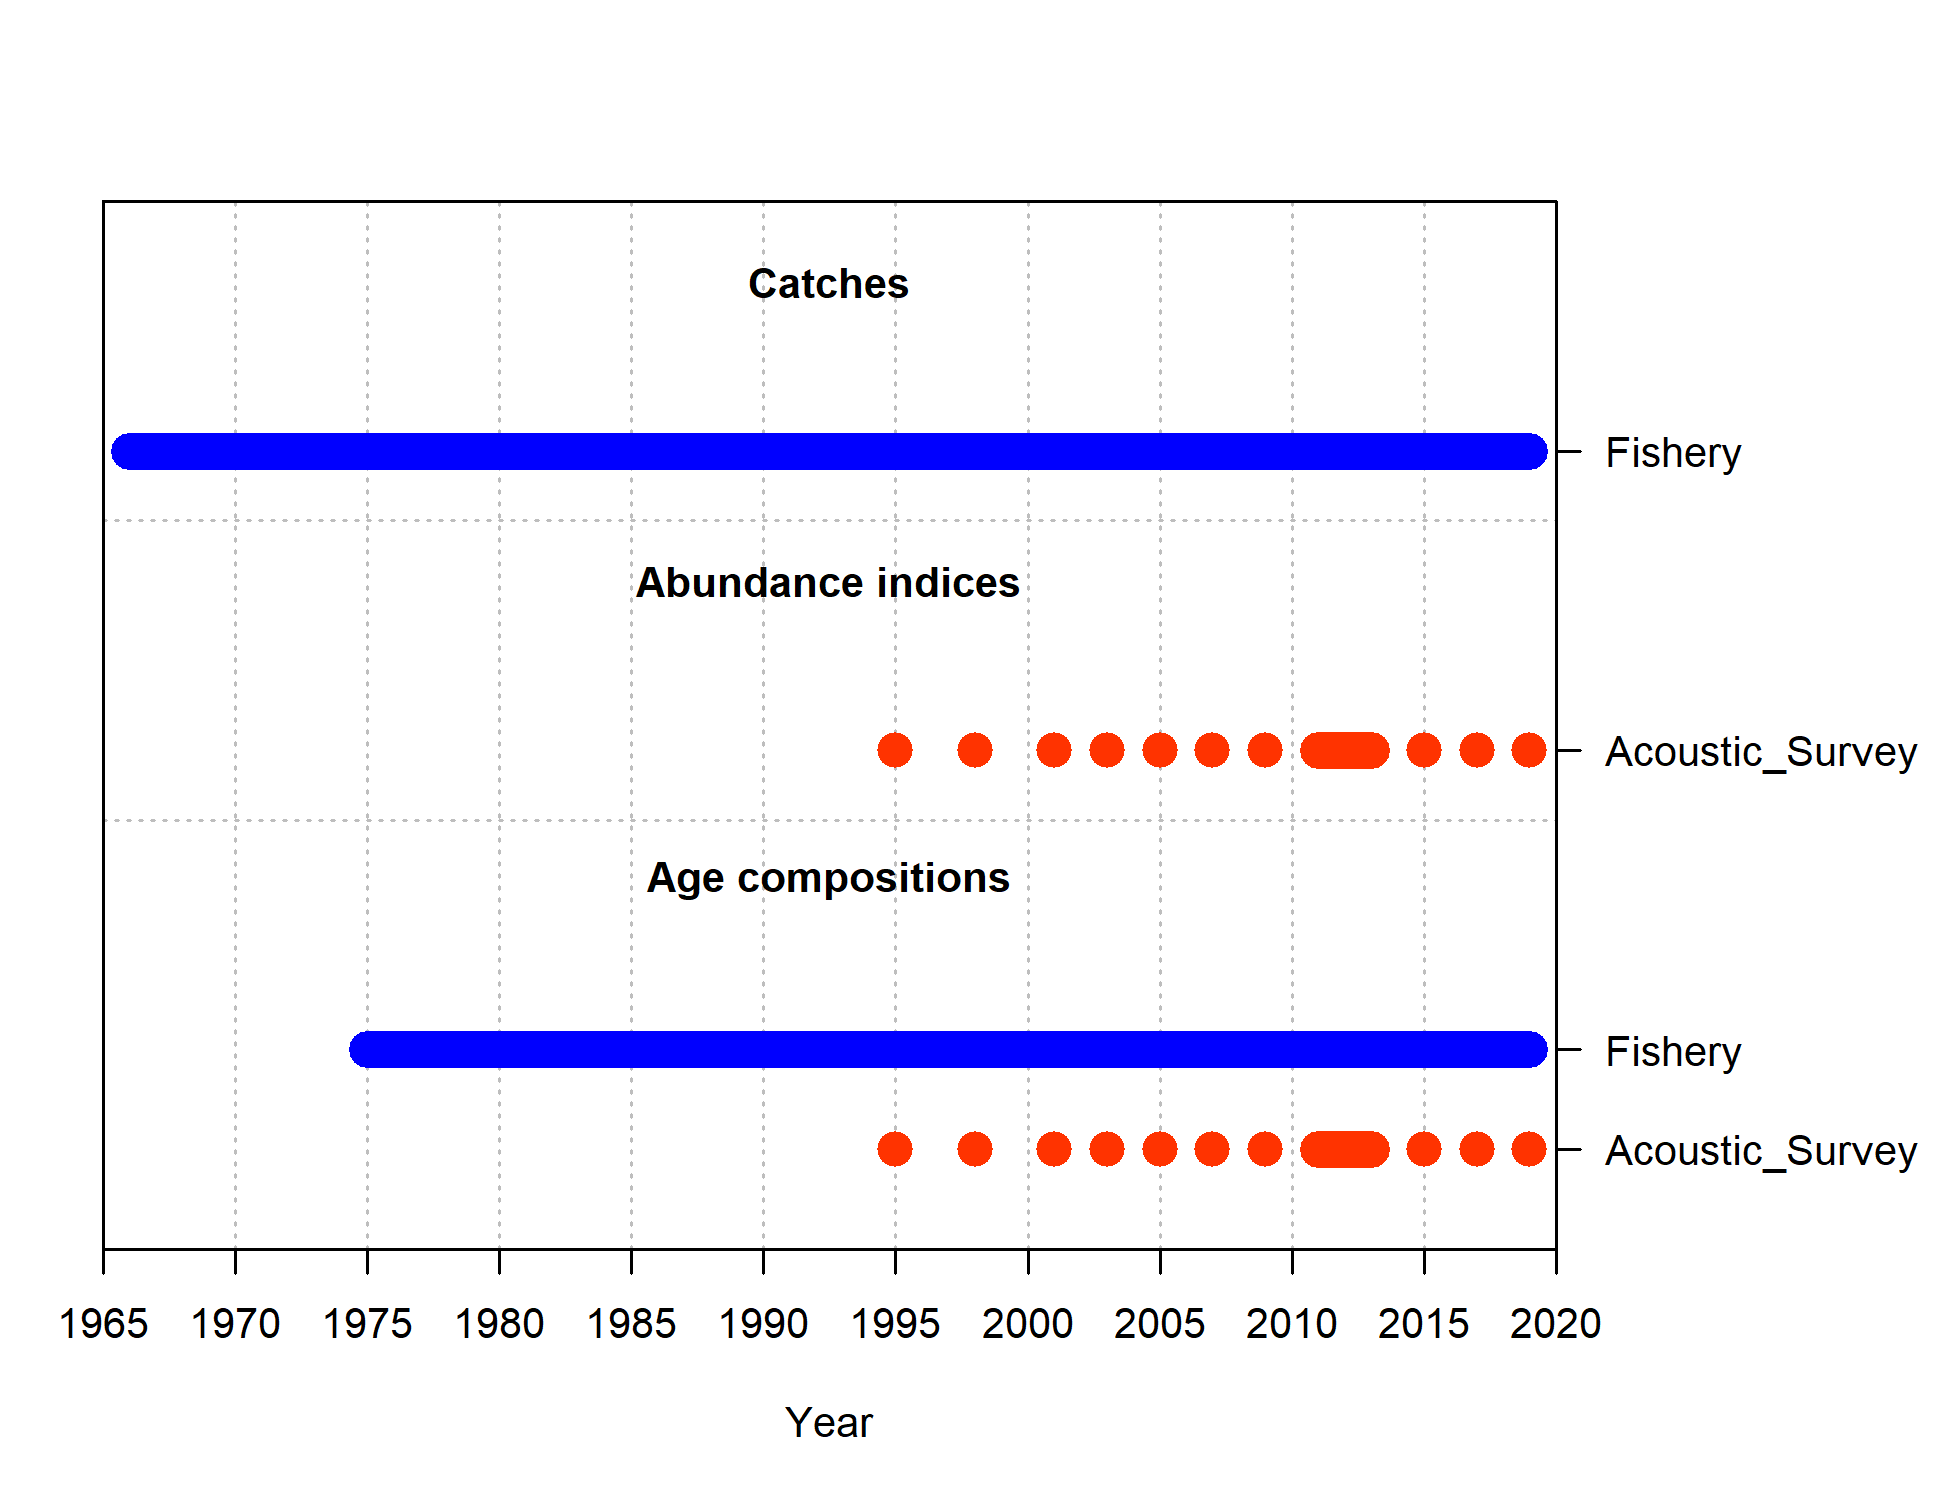
\includegraphics[width=1\textwidth,height=1\textheight]{data-plot.png}
\caption{Summary of data sources used in the base model.\label{fig:data-plot}}
\end{figure}
\end{document}
